% mnras_template.tex
%
% LaTeX template for creating an MNRAS paper
%
% v3.0 released 14 May 2015
% (version numbers match those of mnras.cls)
%
% Copyright (C) Royal Astronomical Society 2015
% Authors:
% Keith T. Smith (Royal Astronomical Society)

% Change log
%
% v3.0 May 2015
%    Renamed to match the new package name
%    Version number matches mnras.cls
%    A few minor tweaks to wording
% v1.0 September 2013
%    Beta testing only - never publicly released
%    First version: a simple (ish) template for creating an MNRAS paper

%%%%%%%%%%%%%%%%%%%%%%%%%%%%%%%%%%%%%%%%%%%%%%%%%%
% Basic setup. Most papers should leave these options alone.
\documentclass[fleqn,usenatbib,letters]{mnras}%added "letters", a4paper is default

% MNRAS is set in Times font. If you don't have this installed (most LaTeX
% installations will be fine) or prefer the old Computer Modern fonts, comment
% out the following line
\usepackage{newtxtext,newtxmath}
% Depending on your LaTeX fonts installation, you might get better results with one of these:
%\usepackage{mathptmx}
%\usepackage{txfonts}

% Use vector fonts, so it zooms properly in on-screen viewing software
% Don't change these lines unless you know what you are doing
\usepackage[T1]{fontenc}
\usepackage{ae,aecompl}


%%%%% AUTHORS - PLACE YOUR OWN PACKAGES HERE %%%%%

% Only include extra packages if you really need them. Common packages are:
\usepackage{graphicx}	% Including figure files
\usepackage{amsmath}	% Advanced maths commands
\usepackage{amssymb}	% Extra maths symbols
\usepackage{cases}  %define a step function

%%%%%%%%%%%%%%%%%%%%%%%%%%%%%%%%%%%%%%%%%%%%%%%%%%

%%%%% AUTHORS - PLACE YOUR OWN COMMANDS HERE %%%%%

% Please keep new commands to a minimum, and use \newcommand not \def to avoid
% overwriting existing commands. Example:
%\newcommand{\pcm}{\,cm$^{-2}$}	% per cm-squared
\newcommand{\FA}{TIC 277539431} %s12
\newcommand{\FB}{TIC 44984200} %s10
\newcommand{\FC}{TIC 237880881} %s1
\newcommand{\FD}{EPIC 212035340} %c18
\newcommand{\FE}{KIC 100004076} %q14
\newcommand{\FF}{TIC 300741820} %s8

%%%%%%%%%%%%%%%%%%%%%%%%%%%%%%%%%%%%%%%%%%%%%%%%%%

%%%%%%%%%%%%%%%%%%% TITLE PAGE %%%%%%%%%%%%%%%%%%%

% Title of the paper, and the short title which is used in the headers.
% Keep the title short and informative.
\title[Where do flares on fully convective dwarfs occur?]{Where do flares on fully convective dwarfs occur?}

% The list of authors, and the short list which is used in the headers.
% If you need two or more lines of authors, add an extra line using \newauthor
\author[E. Ilin et al.]{
E. Ilin$^{1,2}$,\thanks{E-mail: eilin@aip.de}
K. Poppenh\"ager$^{1,2}$,
S. J. Schmidt,$^{1}$,
S. J\"arvinen$^{1}$,
M. Oshagh$^{3,4}$
\\
% List of institutions
$^{1}$Leibniz-Institute for Astrophysics Potsdam (AIP), An der Sternwarte 16, 14482 Potsdam, Germany\\
$^{2}$Institute for Physics and Astronomy, University of Potsdam, Karl-Liebknecht-Str. 24/25, 14476 Potsdam, Germany\\
$^{3}$Instituto de Astrof\'isica de Canarias (IAC), 38205 La Laguna, Tenerife, Spain\\
$^{4}$Departamento de Astrof\'isica, Universidad de La Laguna (ULL), 38206, La Laguna, Tenerife, Spain
}

% These dates will be filled out by the publisher
\date{Accepted XXX. Received YYY; in original form ZZZ}

% Enter the current year, for the copyright statements etc.
\pubyear{2020}

% Don't change these lines
\begin{document}
\label{firstpage}
\pagerange{\pageref{firstpage}--\pageref{lastpage}}
\maketitle

% Abstract of the paper
\begin{abstract}
We report the detection of multiperiod flares on X rapidly spinning fully convective dwarfs in TESS observations. The stars span a range of spectral type from M5 to L1, and rotate at periods between X and X hours. We modeled the flare light curves with a simple flare model light curve that is modified by rotational modulation as the flaring region moves in and out of view. We found that flares on fully convective ultra-fast rotators occur at XXX latitudes.
\end{abstract}

% Select between one and six entries from the list of approved keywords.
% Don't make up new ones.
\begin{keywords}
keyword1 -- keyword2 -- keyword3
\end{keywords}

%%%%%%%%%%%%%%%%%%%%%%%%%%%%%%%%%%%%%%%%%%%%%%%%%%



%%%%%%%%%%%%%%%%% BODY OF PAPER %%%%%%%%%%%%%%%%%%

\section{Introduction}
Magnetic fields are ubiquitous in M dwarfs above, at, and below the mass boundary \citep[$0.35M_\odot$;][]{chabrier1997} between fully convective and partially convective stars~\citep{morin2010, mclean2012}. Stellar flares are magnetic phenomena that occur in all these regimes, and superflares that enhance the optical brightness of a star by orders of magnitude have been detected on stars of all spectral types from solar analogs~\citep{maehara2012} to early L dwarfs~(e.g.,~\citealt{gizis2013}). Relating their properties to rotation and other activity indicators provides unique insights into the nature of these stars' magnetic fields~(e.g.,~\citealt{stelzer2016, paudel2018}).
\\
Stellar flares have been studied in a multitude of wavelengths, albeit rarely simultaneously. With Kepler~\citep{borucki2010} and TESS~\citep{ricker2015}, we are endowed with large monitoring data sets at cadences as high as 1-2 min. We can infer energy budgets, frequencies~\citep{davenport2016, yang2019, guenther2020}, and details about the energy dissipation process from simultaneous spectroscopic observations~\citep{silverberg2016}. However, the location of the flaring region eludes us in the overwhelming majority of cases.
\\
The location of flares is a key piece of information as it constrains the surface field strength and topology: Energetic flares require strong and dynamic magnetic fields that foster re-connection events~\citep{priest2002}. Moreover, the location of flares provides valuable input to dynamo theories: Magnetic field strength and geometry are tightly correlated with rotation~\citep{morin2008, morin2010, vidotto2014, see2019}. Yet the underlying dynamo mechanism that couples the two, both above and below this boundary, remains an open question~(\citealt{wright2018}, and references therein), and would benefit from observational constraints like the magnetically active latitudes of stars with well-known properties.
\\
The location of flares can at least partially explain the variety seen in flare light curve morphologies. The convex shape of a flare light curve in X-rays on V773 Tau~\citep{skinner1997} could be well-described by rotational modulation. Later, effects of rotation and eclipses have been put forward as an explanation for unusual flare light curves multiple times~\citep{stelzer1999,montmerle2000,johnstone2012}. Only few examples of unambiguously located stellar flares exist to date~\citep{wolter2008, peterson2010}.
%A flare loop was detected using radio interferometry near the pole on the K star in the Algol binary system~\citep{peterson2010}.
% Wolter+2008 localized a flare on a K2 near the pole, but not co-located with the spot (rather with the fringes of these regions) using Doppler Imaging
On the Sun, the positions of large flares follow the cyclic latitude variations of sunspots~\citep{zhang2007}. This phenomenon is known as the butterfly diagram, and is crucial to the understanding of the solar dynamo~\citep{gnevyshev1977}% recently observed on a star: Netto (2020)
\\
A particularly intriguing class of objects that exhibit flares are fully convective ultrafast rotating dwarfs (FCUFRs). Their radio and X-ray emission violate the Guedel-Benz~\citep{guedel1993, benz1994} relation, the correlation between the two bands seen in earlier type stars, suggesting a transition in the magnetospheric conditions that govern flaring activity~~\citep{berger2010, mclean2012, cook2014, williams2014}. FCUFRs have rotation periods below a day, often below 12 h. Some are known to exhibit strong magnetic fields, partly exceeding the equipartition value of about 4 kG~\citep{shulyak2017} predicted for the saturated solar-type dynamo magnetic flux~\citep{pevtsov2003}. %These fields give rise to superflares energetic enough to allow us to determine their location on their surfaces from light curves.
\\
The observed morphology of a flare light curve is modulated by the flare's position on the stellar surface relative to the observer during the event~\citep{tovmassian2003}. Energetic superflares can last from less than an hour to over a day~\citep{kowalski2013,paudel2018b}, and so be observable for longer than an entire rotation period if they occur on a sufficiently rapidly rotating star. For favorable inclinations of the rotation axis, we expect to observe a modulation of the intrinsic flare light curve as the active region moves across the visible hemisphere, and disappears or re-appears behind the stellar limb. If the inclination is known, the active region's latitude can be unambiguously determined from this modulation.
\\
We searched for long duration superflares on FCUFR's in Kepler, K2, and TESS light curves and detected a total of five flares showing these modulations. We describe their properties and additional observations in Section \ref{sec:data}. We lay out a simple geometric model that generates signatures of rotationally modulated flares in Section \ref{sec:model}. The fits of our model to the data, and their interpretation are presented in Section \ref{sec:results}. Our concluding remarks and a summary can be found in Section \ref{sec:summary}.
\section{Data and Observations}
\label{sec:data}
We searched the light curves of FCUFRs (spectral types $\sim$M5$-$L2, rotation periods $< 1$ d) in the Kepler, K2, and TESS archives for flares that were visible over multiple rotation periods (Section \ref{sec:photometry}). We found seven candidates of which we chose four events on four different stars for a close investigation. Spectroscopic observations and stellar properties are detailed in Sections \ref{sec:salt} and \ref{sec:props}, respectively.
%-------------------------------------------------------------------
%\begin{table*}
%\caption{Stellar parameters and multiperiod flare observations. Coordinates from~\citet{gaiacollaboration2018}.}
% $a$ is the amplitude of the sine fit to the light curve relative to the median flux.
%\label{tab:observations}
%\begin{tabular}{lccccccr}
\toprule
             ID & QCS &                   other ID & SpT & cadence &        $t_0$ & $P_\mathrm{rot}$ &   $v\sin i$  \\
\midrule
                &     &                            &     &     min &          BJD &                d &        km/s &                s \\
  TIC 277539431 &  12 &  WISEA J105515.71-735611.3 &  M7 &       2 &  2458641.835 &             0.19 &   \\
   TIC 44984200 &  10 &             SCR J0838-5855 &  M6 &       2 &  2458588.030 &            0.113 &   \\
  TIC 237880881 &   1 &    2MASS J01180670-6258591 &  M5 &       2 &  2458331.700 &          0.35125 &   14.4(2.6) \\
 EPIC 212035340 &  18 &    MASS J08371832+2050349  &  M8 &      30 &  2458270.750 &            0.193 &   \\
  KIC 100004076&  14 &  WISEP J190648.47+401106.8 &  L1 &       1 &  2456191.550 &          0.37015$^a$  &   11.2(2.2)\\
\bottomrule


%\hline
%\multicolumn{10}{l}{$^a$ \citet{gizis2013}}\\
%\end{tabular}
%\end{table*}
\subsection{Photometry}
\label{sec:photometry}
We primarily worked with TESS Cycle 1 and Cycle 2 data, but we also went back to the Kepler/K2 archives to search for additional canditates. In this section we explain how we found and curated the photometric data for this study. We list the general properties of all candidates with multi-periodic light curves in Table \ref{tab:properties}. In Section \ref{sec:props} we describe the properties of the subset of these stars that we chose to investigate.
% --------------------------------------------------------
\begin{figure}
	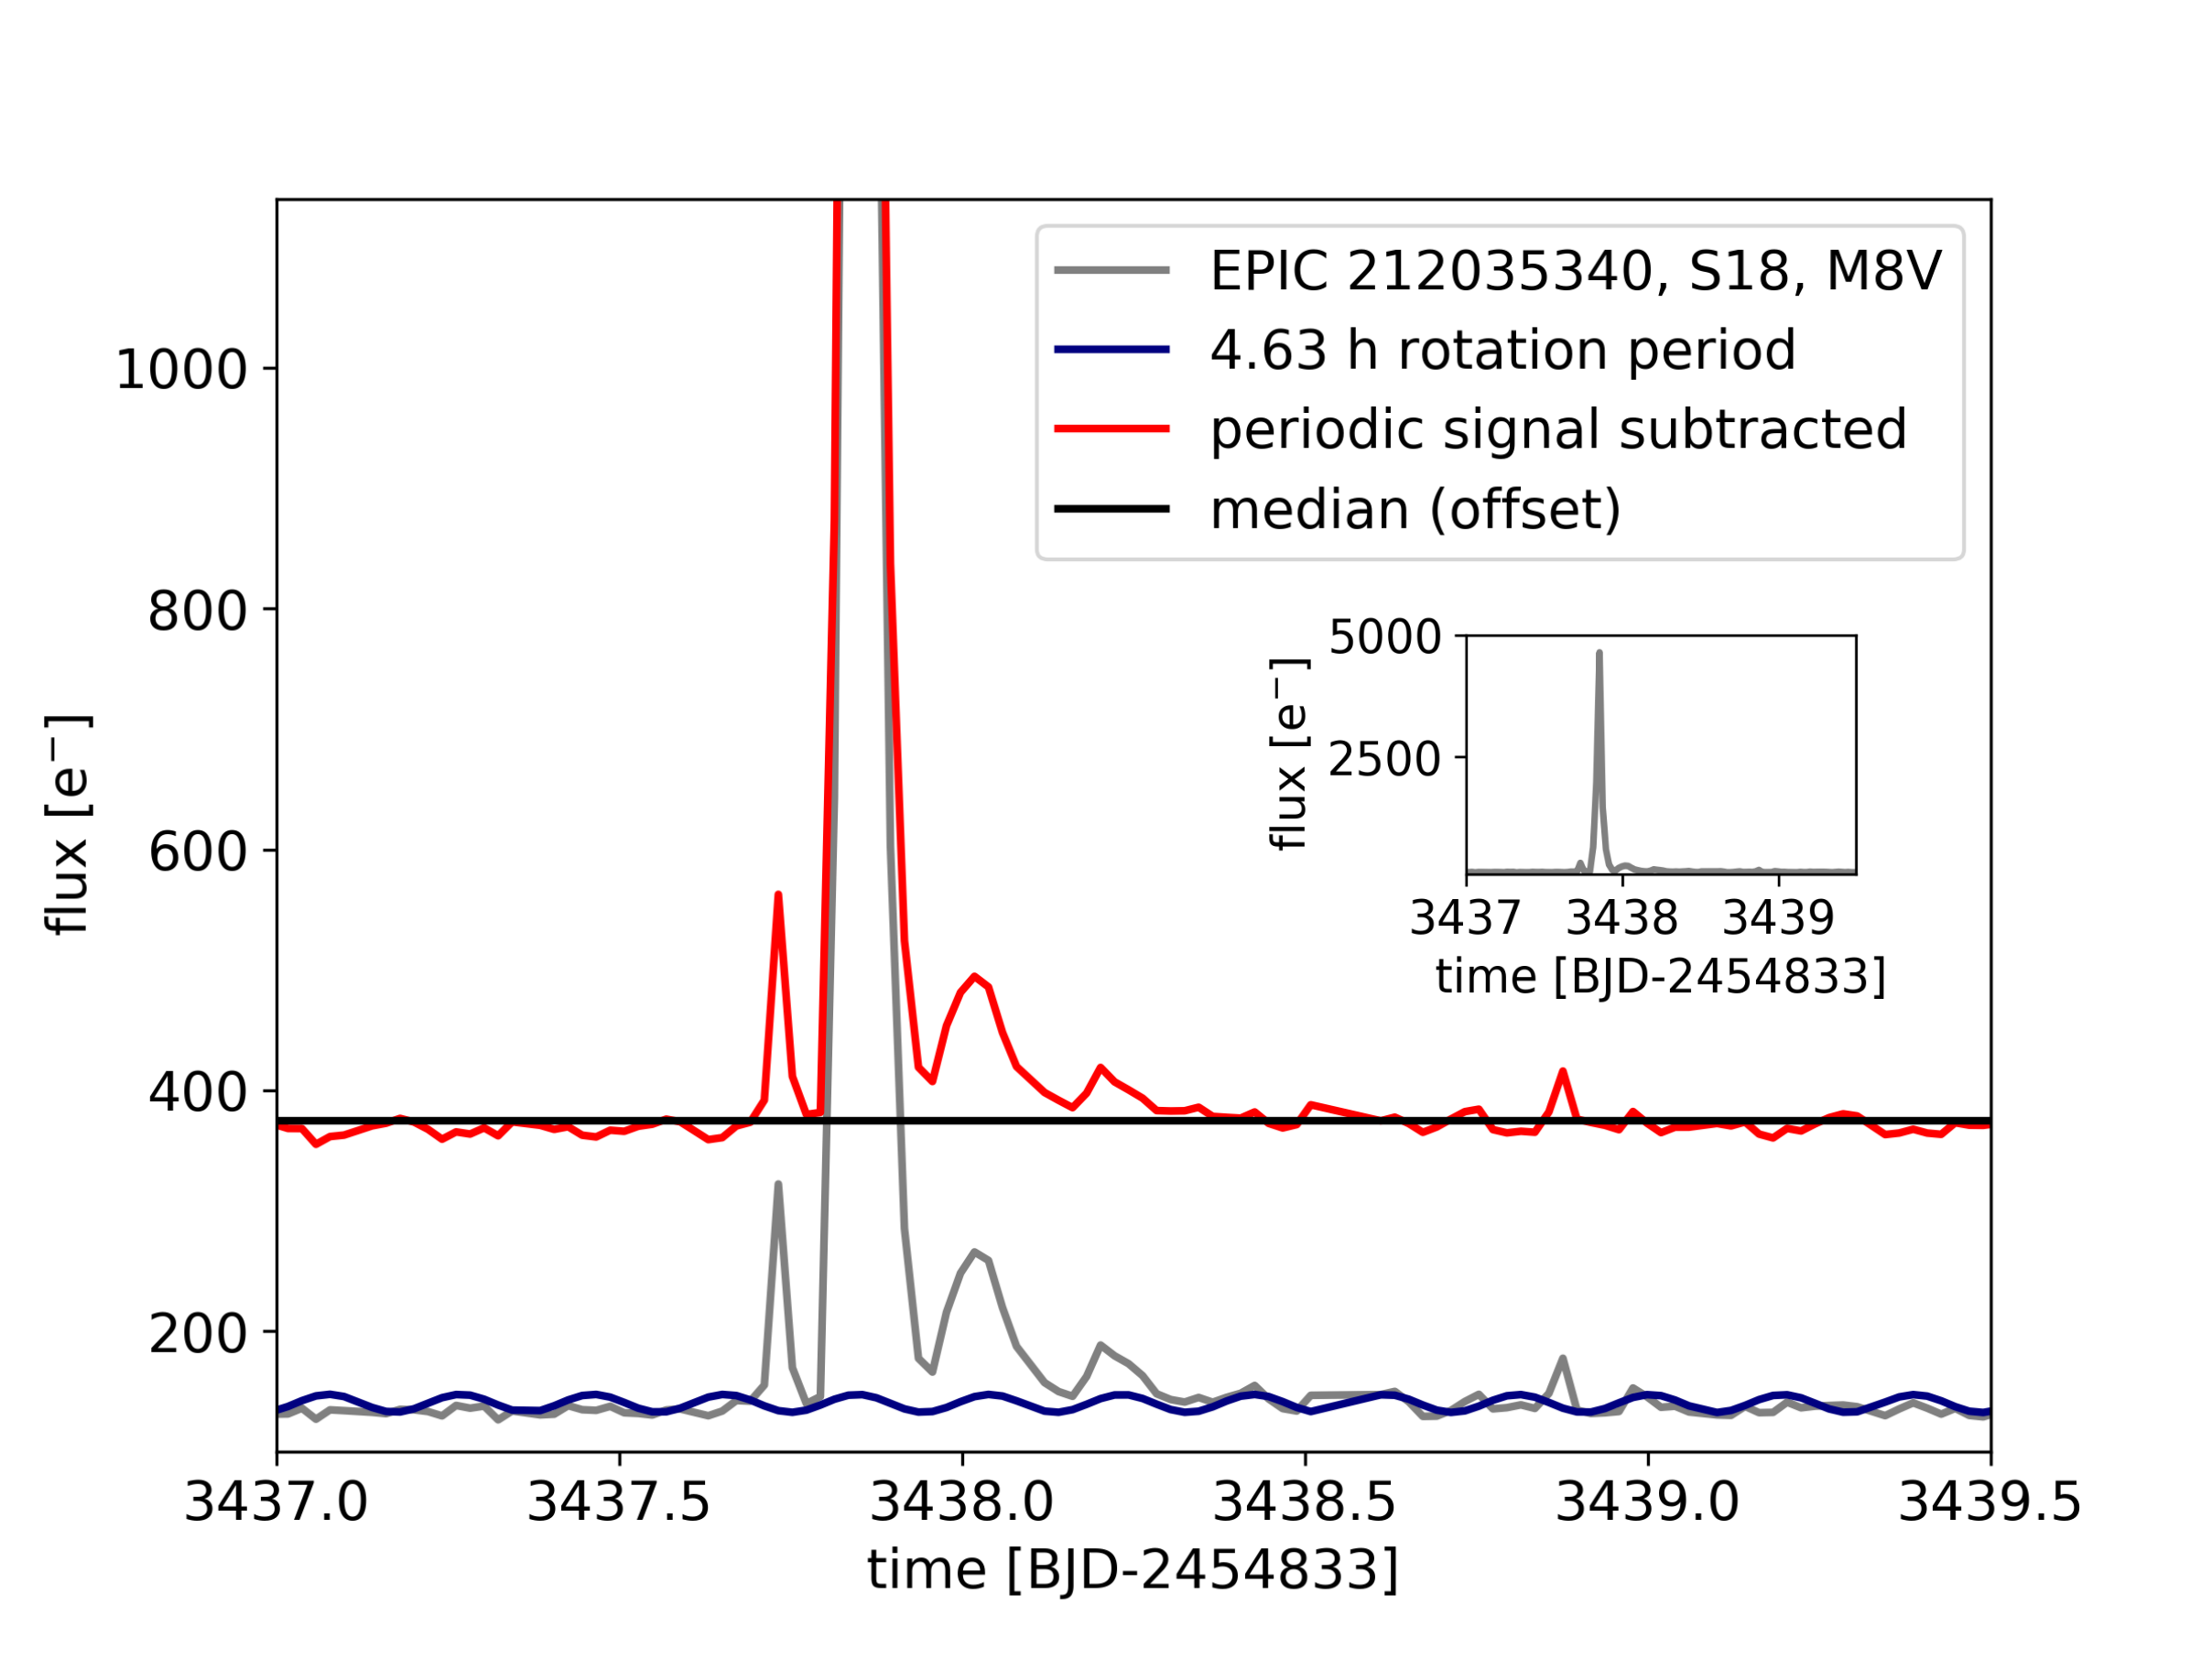
\includegraphics[width=\columnwidth]{figures/EPIC212035340_inset.png}
    \caption{Multiperiod flare in a 30-min cadence light curve of \FD.}
    \label{fig:\FD}
\end{figure}
% --------------------------------------------------------

\subsubsection{Kepler}
\label{sec:photometryKepler}
The Kepler \citep{koch2010} satellite obtained high precision photometric observations of thousands of stars in the Cygnus-Lyra region during its primary mission between 2009 and 2013. Besides being the most successful exoplanet finder mission to date, it has greatly advanced the research of physics of cool stars. For instance, the continuous monitoring at 1-minute cadence enabled the detection of energetic stellar flares on stars that were previously classified inactive from ground-based observations.
\\
However
%, there was no dedicated program to observe stars with spectral type later than M6 (ultracool dwarfs, UCDs,~\citealt{kirkpatrick1997}) with Kepler. O
only one FCUFR, an L1 dwarf, WISEP J190848.47+401106.8, or \FE, was monitored during Quarters 10-17 in 30-minute cadence, and during Quarter 14 in 1-minute cadence. It showed very stable rotation with $P=8.9$ h~\citep{gizis2013}, 
%It has different designations in each quarter: KIC 100003560 (Quarter 10), KIC 100003605 (Quarter 11), KIC100003905 (Quarter 12), KIC 100004035 (Quarter 13), and KIC100004076 (Quarter 14).
and a long-duration flare occurred in the 1-minute cadence \texttt{PDCSAP\_FLUX} light curve in Quarter 14~(Fig.~\ref{fig:fit\FE}).
\subsubsection{K2}
\label{sec:photometryK2}
From 2013, when two of Kepler's reaction wheels failed, and the mission was recast as K2~\citep{howell2014}, until the spacecraft ran out of fuel in 2018, almost 20 $\sim$80
days long observation campaigns were conducted in varying fields of view nearby the ecliptic plane. Despite its reduced pointing accuracy, K2 has observed hundreds of thousands of stars (albeit for a shorter period than Kepler), including a number of FCUFRs.
\\
Targeted observations of fully convective dwarfs took place throughout the mission~\citep{gizis2017, gizis2017b, paudel2018} but no peculiar events took place.
%The first object with a superflare that was visible for 15.4 h in this series, EPIC 220186653 (Campaign 8, 30-minute cadence), an L1 dwarf, did not show any periodic modulation~\citep{gizis2017}. In a further study, two out of three UCDs were found flaring, but no long-duration flares took place during the observations~\citep{gizis2017b}. From the K2 UCDs studied in~\citet{paudel2018} three showed rotational modulation below 0.5 days, and exhibited impulsive short duration flares, but no long duration events.
%\\
In the study of three rapidly rotating UCDs in K2 long cadence light curves~\citep{paudel2019}, %EPIC 212027121 showed one flare in C18 that spans almost one rotation period without a clear modulation; EPIC 212136544 showed three flares in C18, each with a double peak structure on time scales comparable to its photometric period of about 7 hours; and
\FD~(Campaign 18) showed a flare that was visible for at least three periods of about 4.6 hours.
While
%EPIC 212136544, and especially
\FD~showed intriguing morphology~(Fig. \ref{fig:\FD}), we did not investigate this case further here because its light curve was obtained in 30-minute cadence, that is, of lower quality than the rest of our sample, and the target was very faint ($J\approx 16$) and thus challenging for high-resolution spectroscopy that would have been needed to determine the inclination of its rotation axis.
%The periodic modulation we find has nothing to do with the quasi-periodic oscillations observed for two large flares on Proxima Cen because its rotation period is about 83 days~\citep{vida2019}.
\subsubsection{TESS}
\label{sec:photometryTESS}
The Transiting Exoplanet Survey Satellite, (TESS, \citealt{ricker2015}) is Kepler's successor mission. Its goal is to observe the full sky of stars brighter than $\sim13$ mag in 2-minute or 30-minute cadence for at least $\sim$27 days each to detect planetary candidates for follow-up observations with the James Webb Space Telescope~\citep{gardner2006}. Just as with Kepler, the obtained light curves contain valuable information not only about exoplanets but also about the stars themselves, and their flaring activity in particular. However, the TESS band ranges from the red optical to the near infrared~($6000-10000$\AA), whereas the Kepler band was centered in the optical between $4200$\AA\; and $9000$\AA. 
\\
Our primary source of long duration flares on FCUFRs observed during TESS Cycle 1 (Southern hemisphere) and Cycle 2 (Northern hemisphere, Sectors 14, 15, and 16) was the G022164 guest observer program led by J. Sebastian Pineda ("Exploring The Variability Of Ultracool Dwarfs With TESS"). We searched a total of 191+74 $\sim 27$ day long light curves obtained at 2-minute cadence on 110+32 targets for rotational modulation and long duration flares, and found two candidates, \FA~(Sector 12) and \FB~(Sector 10).
\\
To complement our sample with dwarfs of types M5 and M6, we searched the sample of rapidly rotating M dwarfs with rotation periods below 4 h in TESS sectors 1 and 2 from ~\citet{zhan2019} and the M dwarf flare star sample in TESS Sectors 1-3 with rotation periods below 10 hours from~\citet{doyle2019} for flares. We found a long duration flare in \FF, Sector 8, an M6 dwarf that showed rotational modulation at 3.17 h, and a complex, long-duration flare on \FC, and M5 dwarf observed during Sector 1 with a rotation period of 8.43 h.
\subsection{Spectroscopy}
\label{sec:salt}
\subsubsection{SALT Observations and Data Reduction}
\textcolor{r}{\textbf{Katja SALT observations}}
\\
Data reduction was done with the PEPSI data reduction software. The detailed description is given in
\citet{2018Strassmeier}.
It relies on adaptive selection of parameters by using statistical inference
and robust estimators. Shortly, the standard reduction steps include bias overscan
detection and subtraction, scattered light extraction from the inter-order
space and subtraction, definition of \'echelle orders, optimal extraction of
spectral orders, wavelength calibration, and a self-consistent continuum fit
to the full two-dimensional (2D) image of extracted orders.
\subsubsection{$v\sin i$}
\label{subsec:vsini}

% --------------------------------------------------------
\begin{figure}
	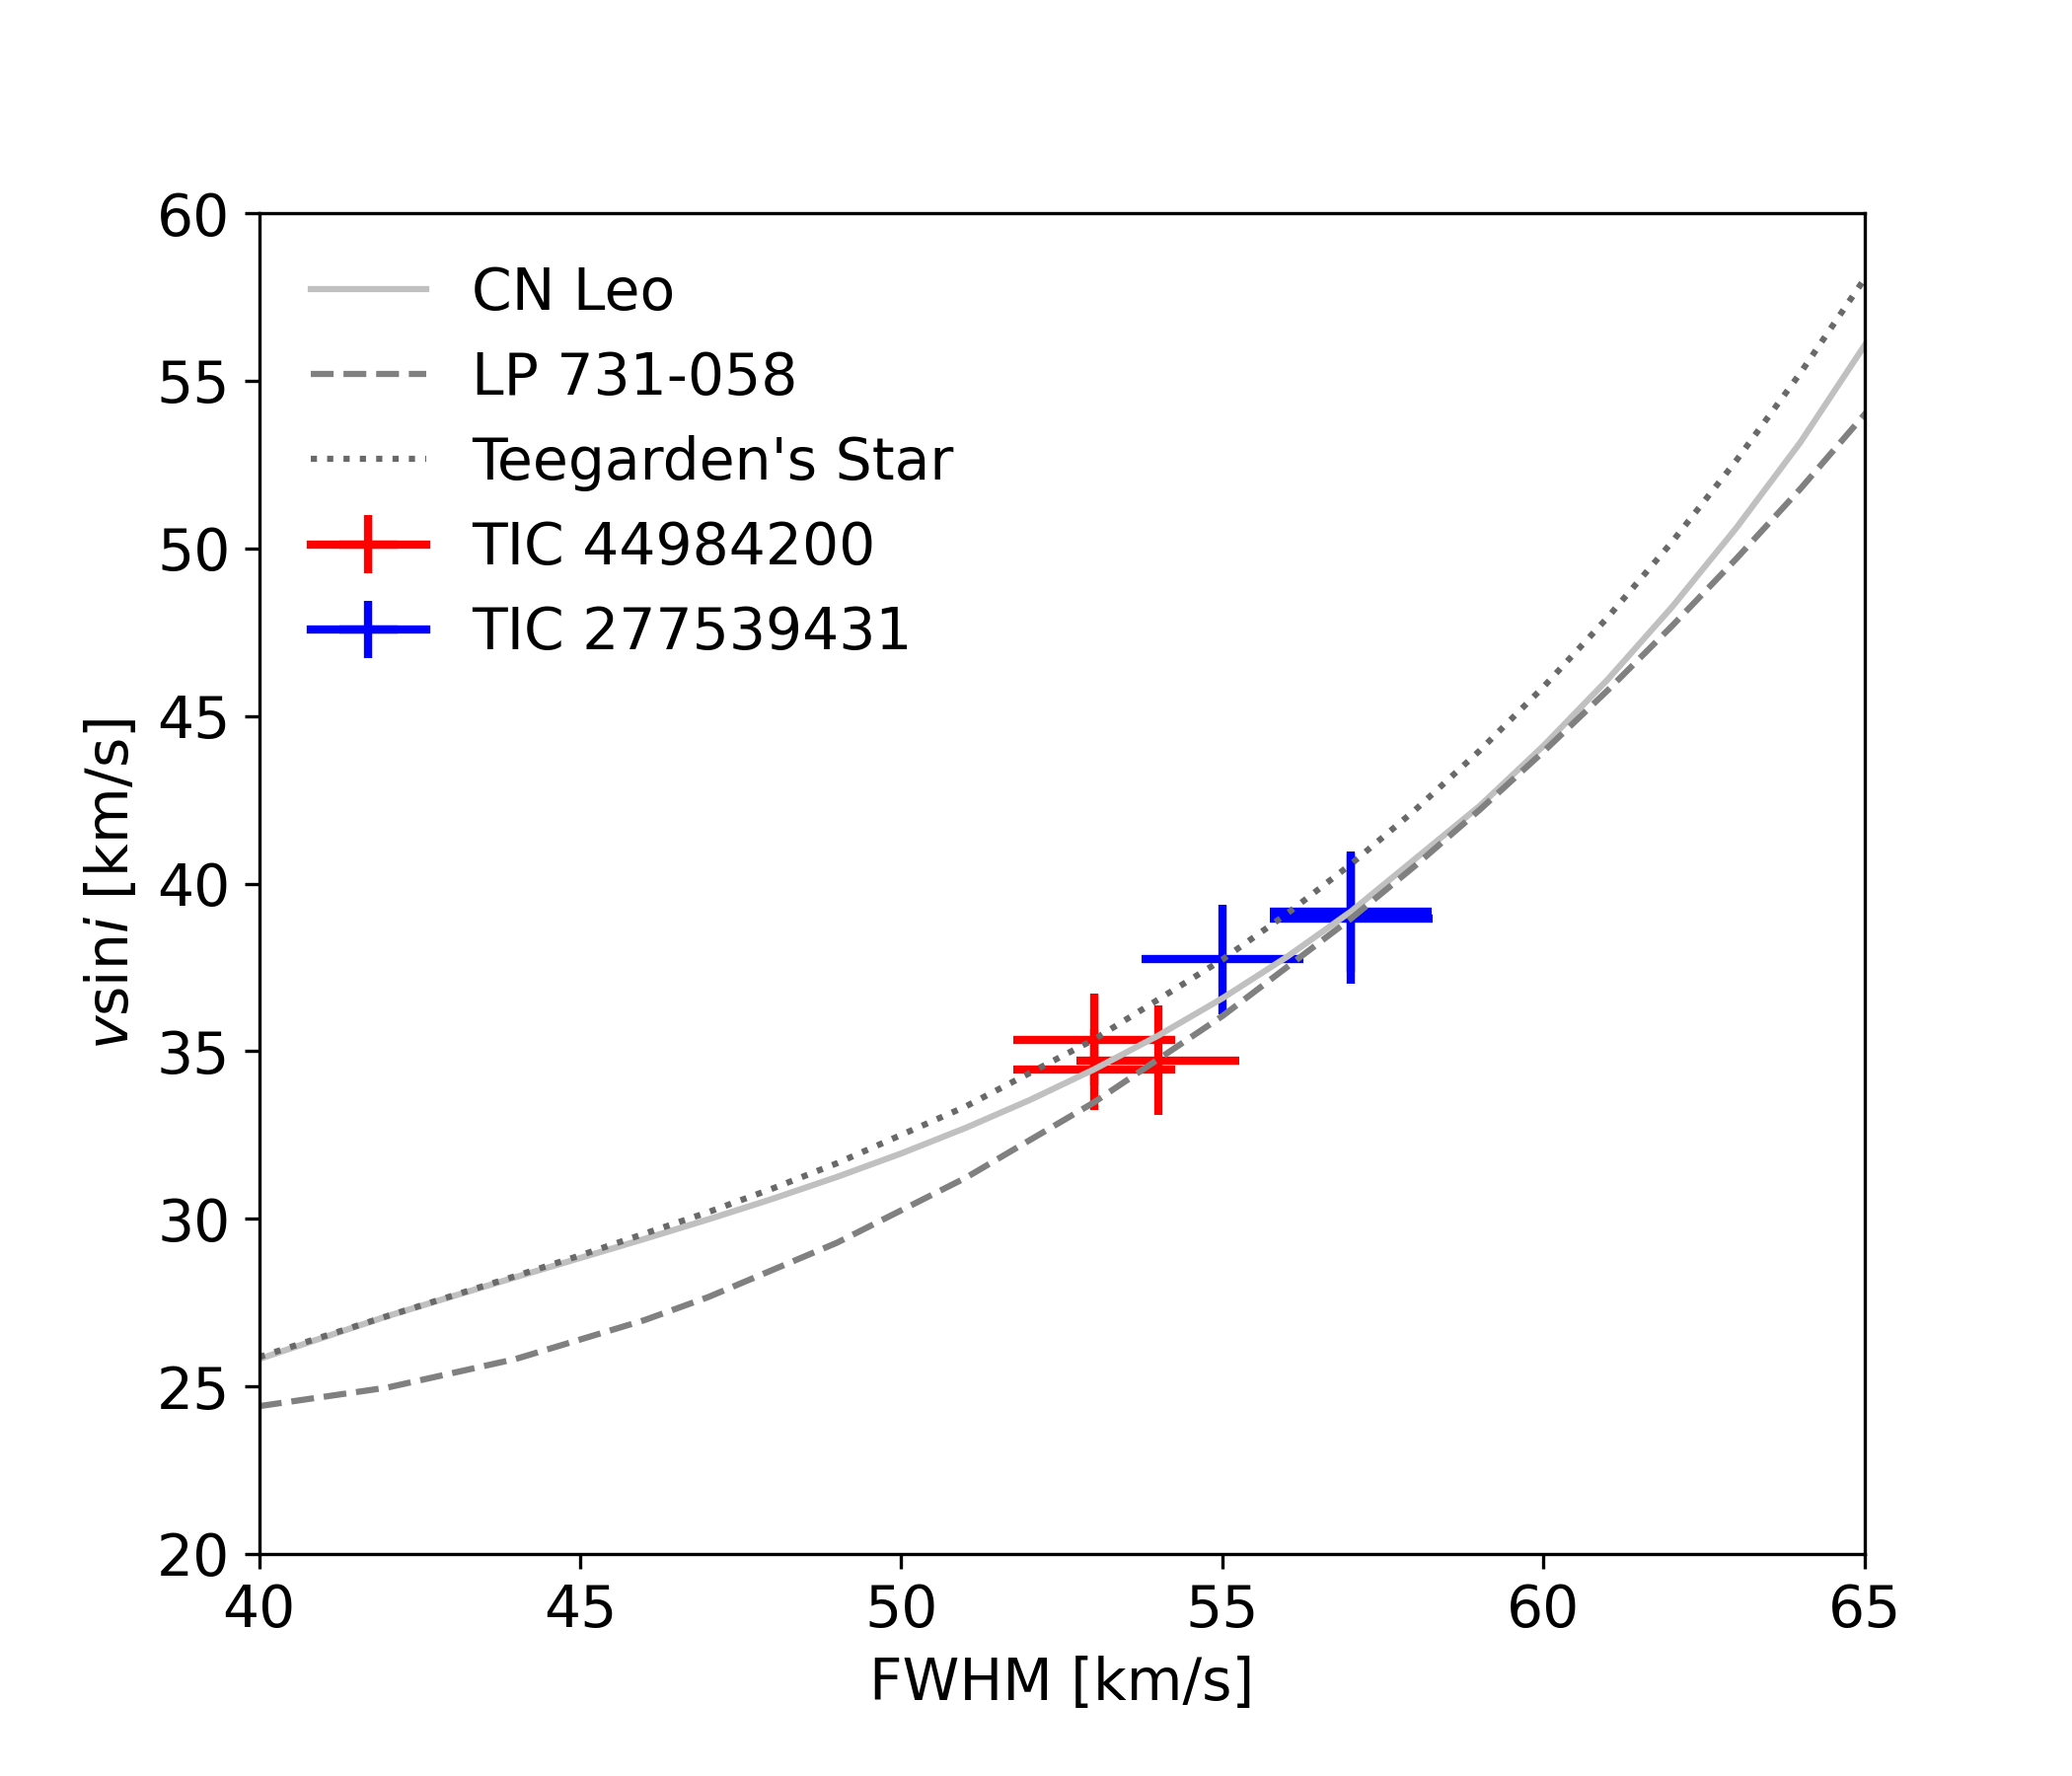
\includegraphics[width=\columnwidth]{figures/vsini.png}
    \caption{Grey lines: Third order polynomial fits to the calibration functions for three different template spectra. Blue and red crosses: Fitted FWHM from the CCFs of SALT spectra with uncertainties.}
    \label{fig:vsini}
\end{figure}
% --------------------------------------------------------

For the $v\sin i$ inference we followed the cross-correlation procedure detailed in \citet{reiners2012}.
The technique uses the cross-correlation functions~(CCF) of rotationally broadened template spectra to calibrate a relation between the FWHM of the CCF and $v\sin i$. We calibrated the normalized CCF using high-resolution optical CARMENES spectra of CN Leo (M6), LP 731-058 (M6.5), and Teegarden's Star (M7) for which~\citet{reiners2018} determined $v\sin i < 3$ km/s using the same method but different reference stars, and utilizing different parts of the spectrum. We broadened these three template spectra using the \texttt{eniric}~\citep{neal2019} software assuming a limb darkening coefficient $\epsilon=0.6$ in the range from $1$ to $60$ km/s with a resolution of $1$ km/s. Then we measured the FWHM to derive a calibration function for $v\sin i$.
\\
After inspecting the observed SALT spectra and the template CARMENES spectra, and experimenting with various regions in the red part of each spectrum we found the region $7938-7955$\AA\; surrounding the Rb 7948\AA\; line to be uniquely suited for the technique, as it was a strong line largely unaffected by telluric features which was most sensitive to changes in $v\sin i$ in the $10-50$ km/s range. The lower bound for our uncertainty is given by the resolution of our spectra and the sensitivity of FWHM to changes in $v\sin i$. We fit a 3rd order polynomial to the calibration function, and use the fit to propagate the uncertainty on FWHM to the resulting $v\sin i$ values~(Fig. \ref{fig:vsini}). We found uncertainties on $v\sin i$ in the $1.2-1.9$ km/s range for individual pairs of templates and spectra. Taking the average of all three templates the uncertainty naturally decreased to $0.8-1.0$ km/s.
\\
We validated our results by comparing with randomly chosen spectra at $v\sin i$ between $14$ km/s and $42$ km/s that had high-resolution optical spectra~\citep{reiners2018} listed in the CARMENES input catalog~\citep{jeffers2018}\footnote{Spectra publicly available on \url{http://carmenes.cab.inta-csic.es/gto/jsp/reinersetal2018.jsp}}. We found them consistent with our fits within uncertainties. From these comparisons we estimated our uncertainty on individual $v\sin i$ to be $\approx 3$ km/s.
%eniric
%xcorr for cross-correlation https://github.com/trichter/xcorr/blob/master/xcorr.py
% spt of templates, vsini of templates
%-----------------------------------------


\begin{table*}
\centering
\caption{Properties of stars with multi-period flares.}
\label{tab:properties}
\begin{tabular}{ccccccc}
\hline\hline
TESS/Kepler ID & 2MASS ID & ST & Gaia G & J & K$_S$ & Distance (pc) \\
\hline
TIC 237880881&01180670-6258591 & M5 & 14.98 & 11.53 & 10.64 & 46.1$\pm$0.1 \\
TIC 300741820&07404497-6648318 & M6 & 15.33 & 11.96 & 11.13 & 22.3$\pm$4.4 \\
%EPIC 212035340&08371832+2050349 & M8 & 19.57 & 15.89 & 14.88 & 103.6$\pm$20.5 \\
TIC 44984200&08380224-5855583 & M6 & 14.41 & 10.31 & 9.27 & 11.1$\pm$0.0 \\
TIC 277539431&10551532-7356091 & M7 & 14.74 & 10.63 & 9.67 & 13.7$\pm$0.1 \\
KIC 100004076&19064801+4011089 & L1 & 17.84 & 13.08 & 11.77 & 16.8$\pm$0.0 \\
\hline
\end{tabular}


\end{table*}


\begin{table}
\centering
\caption{Rotation and inclination of stars with multi-period flares.}
\label{tab:geometry}
\begin{tabular}{lcccr}
\hline\hline
      ID &    $P$ (h) & $v \sin i$ (km/s) &    $i$ (deg) &     $v\sin i$ ref. \\
\hline
 TIC 237 &  8.4(0.03) &       $14.4(2.6)$ &  $21.3(2.3)$ &  \citet{kraus2014} \\
 TIC 449 &  2.7(0.03) &       $34.8(3.0)$ &  $33.1(1.6)$ &          this work \\
 TIC 277 &  4.6(0.03) &       $38.6(3.0)$ &  $87.1(2.4)$ &          this work \\
 KIC 100 &  8.9(0.00) &       $11.2(2.2)$ &  $57.4(6.5)$ &  \citet{gizis2013} \\
\hline

\end{tabular}

\end{table}
\subsection{Stellar Properties}
\label{sec:props}
To understand the flares and place them in context, we characterized the stars they occurred on. We adopted spectral types from previous work that assigned types based on low-resolution optical spectroscopy (cite either here or in table).

We cross-matched the list of six targets to the Two Micron All-Sky Survey \citep[2MASS;][]{Skrutskie2006} and Gaia \citep{gaiacollaboration2016} DR2 database \citep{gaiacollaboration2018} to obtain optical and infrared photometry and parallax distances. We used a cross-match radius of 10\arcsec, selecting the nearest match in each survey if more than one object fell within the matching radius. For the five objects with parallaxes in Gaia DR2, we adopt the inverse parallax as distance. For \FF, the excess of the astrometric noise was too high to use the parallax, so we calculated a distance based on the relationship between absolute $K_S$ and spectral type from \citet{dupuy2012}.

We calculated radii based on the relationship between absolute $K_S$ magnitude and radius from \citet{Mann2015}. The uncertainties are based on a combination of the scatter in the relationship $\sim3$\% and the uncertainties on distance and $K_S$ magnitude.

The lightcurves provided by TESS and Kepler do not have accurately calibrated absolute fluxes that are needed to characterize the energy of the flares. We calculate quiescent fluxes in the TESS and Kepler bands using their spectrophotometry. We first construct representative spectra for each spectral type that cover the TESS-Kepler-Gaia range (give numbers here) by combining the spectroscopic templates of \citet{Bochanski2007} and \citet{Schmidt2014a} and IR prism spectra from the spex prism library (cite). We then integrate over the Gaia lightcurve and normalize the SED to the Gaia value. To obtain fluxes in Kepler and TESS, we integrate over the response curves provided by each survey.

The major uncertainty in the spectrophotometric fluxes is the underlying spectral energy distribution, so we assign uncertainties to the fluxes based on the fluxes calculated from the same Gaia flux but with a difference of one spectral type. We then converted flux to luminosity using the distances.

Introduce $F_{f,s}(T_f)$ and $L_{s,q}$ (see Section \ref{ssec:flaringregion})

Most info goes into Table~\ref{tab:stars} but we provide some details on individual targets below:

\subsubsection{\FF}
\label{sec:propsF}
% TIC 300
% --------------------------------------------------------
\begin{figure}
	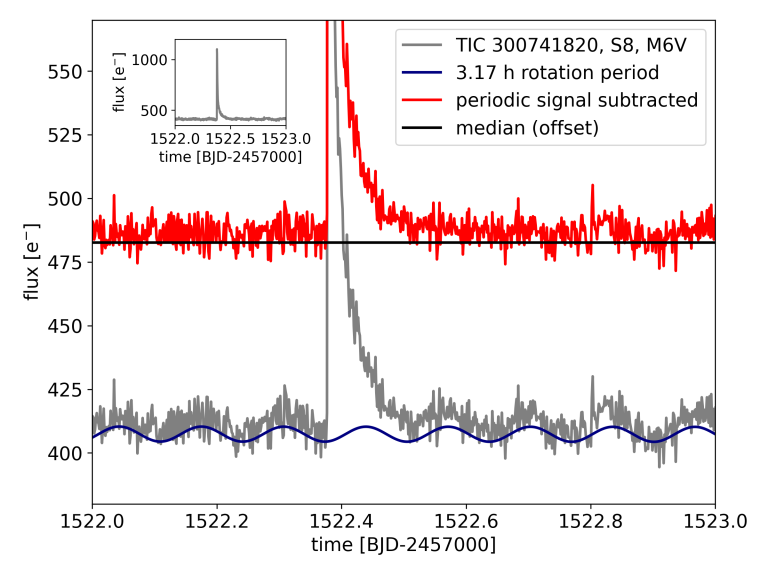
\includegraphics[width=\columnwidth]{figures/EPIC300741820_inset.png}
    \caption{Multi-period flare on \FF. Although the total duration of the flare covered more than a full rotation period, no significant modulation is observed. We could not derive the inclination from the SALT spectrum of \FF, but its astrometric properties suggest that it is an unresolved astrometric binary (see Section \ref{sec:propsF}).}
    \label{fig:\FF}
\end{figure}
% --------------------------------------------------------
Before being revealed to be an FCUFR ($P=3.17$ h) by TESS~\citep{zhan2019}, \FF\,~(UCAC4 116-015389) has not been in scientific spotlight despite its relative brightness (K$_s\approx11$) and proximity ($d\approx22$ pc). In fact, its observables are peculiar in many ways. The SALT spectrum we obtained for \FF\; showed only weak lines, and none appeared to be suited for $v \sin i$ calculation. For instance, the Rb line was fairly weak. We found that the astrometric excess noise $\epsilon_i$ in the Gaia DR2 solution was $7$\,mas, and had a significance of $D\approx6780$. $D$ is indicative of strong disagreement between the Gaia observations, and the best-fitting standard astrometric model. $D>2$ can be interpreted as a sign of unresolved binarity or exoplanets~\citep{lindegren2012}. In certain cases, $\epsilon_i$ can be used to infer the orbital inclination of the system~\citep{kiefer2019a, kiefer2019b}. The K$_s$ magnitude yielded spectral type M6, but the spectrum was more indicative of an earlier spectral type. Moreover, WISE color $W1-W2$ indicated M6, but 2MASS $J-K$ was consistent with spectral type M4~\citep{pecaut2013}. While weak lines could indicate low metallicity, the high astrometric excess noise suggests that \FF\; is a binary system in a close to pole-on orbit. Assuming that rotational modulation and the observed flare stem from the same component, and that the rotation axis of that star is reasonably aligned with the orbital axis, multi-period flares occurring on its surface should be weakly modulated. This is the case for the observed multi-period flare~(Fig.~\ref{fig:\FF}). The notion that stellar rotation is well aligned with the rotational axes of stellar and planetary companions because they stem from the same rotating disc was put in question by a growing number of misaligned binaries~(\textbf{citation}), and exoplanet systems with Hot Jupiters~\citep{winn2015} that suggested that formation histories are more turbulent in general than previously thought. However, in fully convective low-mass stars spin-orbit alignment is poorly constrained with only a few known systems~\citep{konopacky2012, harding2013, zhang2020}.

\subsubsection{\FC}
\label{sec:propsC}
%TIC 237
\FC\;(2MASS J01180670-6258591) is our earlierst type FCUFR, an M5 dwarf at a distance of 46 pc. Its Gaia DR 2 astrometric solution yields a 76\% membership of the Tucana-Horologium association~\citep{ujjwal2020}, a young nearby moving group with age estimates spanning $4-45$\;Myr~\citep{ujjwal2020, bell2015, kraus2014}. We measured a rotation period of 8.43 h in its TESS light curve, and used the catalogued $v\sin i=14.4\pm2.6$ km/s~\citep{kraus2014} to derive an inclination of $21.3\pm2.3$ degrees. 
\subsubsection{\FB}
\label{sec:propsB}
%TIC 449
\FB\;was first discovered as the high proper motion star SCR J0838-5855~\citep{finch2007}. It is an M6 dwarf 11.1 pc away rotating at $P=2.71$ h. Using the method described in Section \ref{subsec:vsini}, we derived $v\sin i=$\input{values/449_vsini.txt} for \FB, and an inclination of $33.1\pm1.6$ degrees. 

\subsubsection{\FA}
\label{sec:propsA}
%TIC 277
\FA\; is an M7 dwarf 13.7 pc away. The dominating peak in the periodogram of its TESS light curve was at 4.56 h with a secondary peak at half of this period. Since the flare signal was modulated by the longer period, we adopted it as the rotation period of the star. Using the method described in Section \ref{subsec:vsini}, we derived $v\sin i=$\input{values/277_vsini.txt} for \FA, and a high inclination of about $87.1\pm2.4$ degrees. 

\subsubsection{\FE}
\label{sec:propsE}
% KIC 100
\FE\; is the latest type specimen in our sample, an L1 dwarf observed by the original Kepler mission. Its light curve showed a very stable 8.9 h rotation period throughout the five Quarters of Kepler observations, exhibits flares, and it had measured H$\alpha$ emission~\citep{gizis2013}, and remained stable during two years of Kepler monitoring despite some minor changes in the shape of the phased curves in later Quarters compared to the earlier ones~\citep{gizis2015}. The lack of this variability at 4.5$\mathrm{\mu}$m suggests that the "spot" that dominates the modulation is in fact a cloud, similar to the Great Red Spot\citep{gizis2015}. \citet{gizis2013} obtained $v\sin i = 11.2\pm2.2$ km/s by fitting a parametrized model to a near-infrared spectrum of \FE, and used it to derive a median inclination of 56 degrees with a heavy tail towards higher inclinations (5th and 95th percentile at 50 and 78 deg, respectively). They used a distance of $16.35 \pm^{0.36}_{0.34}$ pc from ground based parallax measurements. We reproduced their analysis with the improved Gaia distance of $16.8\pm0.04$ pc, and found $i=57.4 \pm 6.5$ deg. As in \citet{gizis2013}, the main source of uncertainty was $v\sin i$, but the tail was less heavy (5th and 95th percentiles of the posterior distribution were at 48 and 73 deg, respectively).
% 18_08_2020_KIC1000_MCMC_uninformative_gaia_2800_steps.csv for 72.3 degrees

%-------------------------------------
\section{Flare modulation model}
\label{sec:model}
% --------------------------------------------------------
\begin{figure*}
	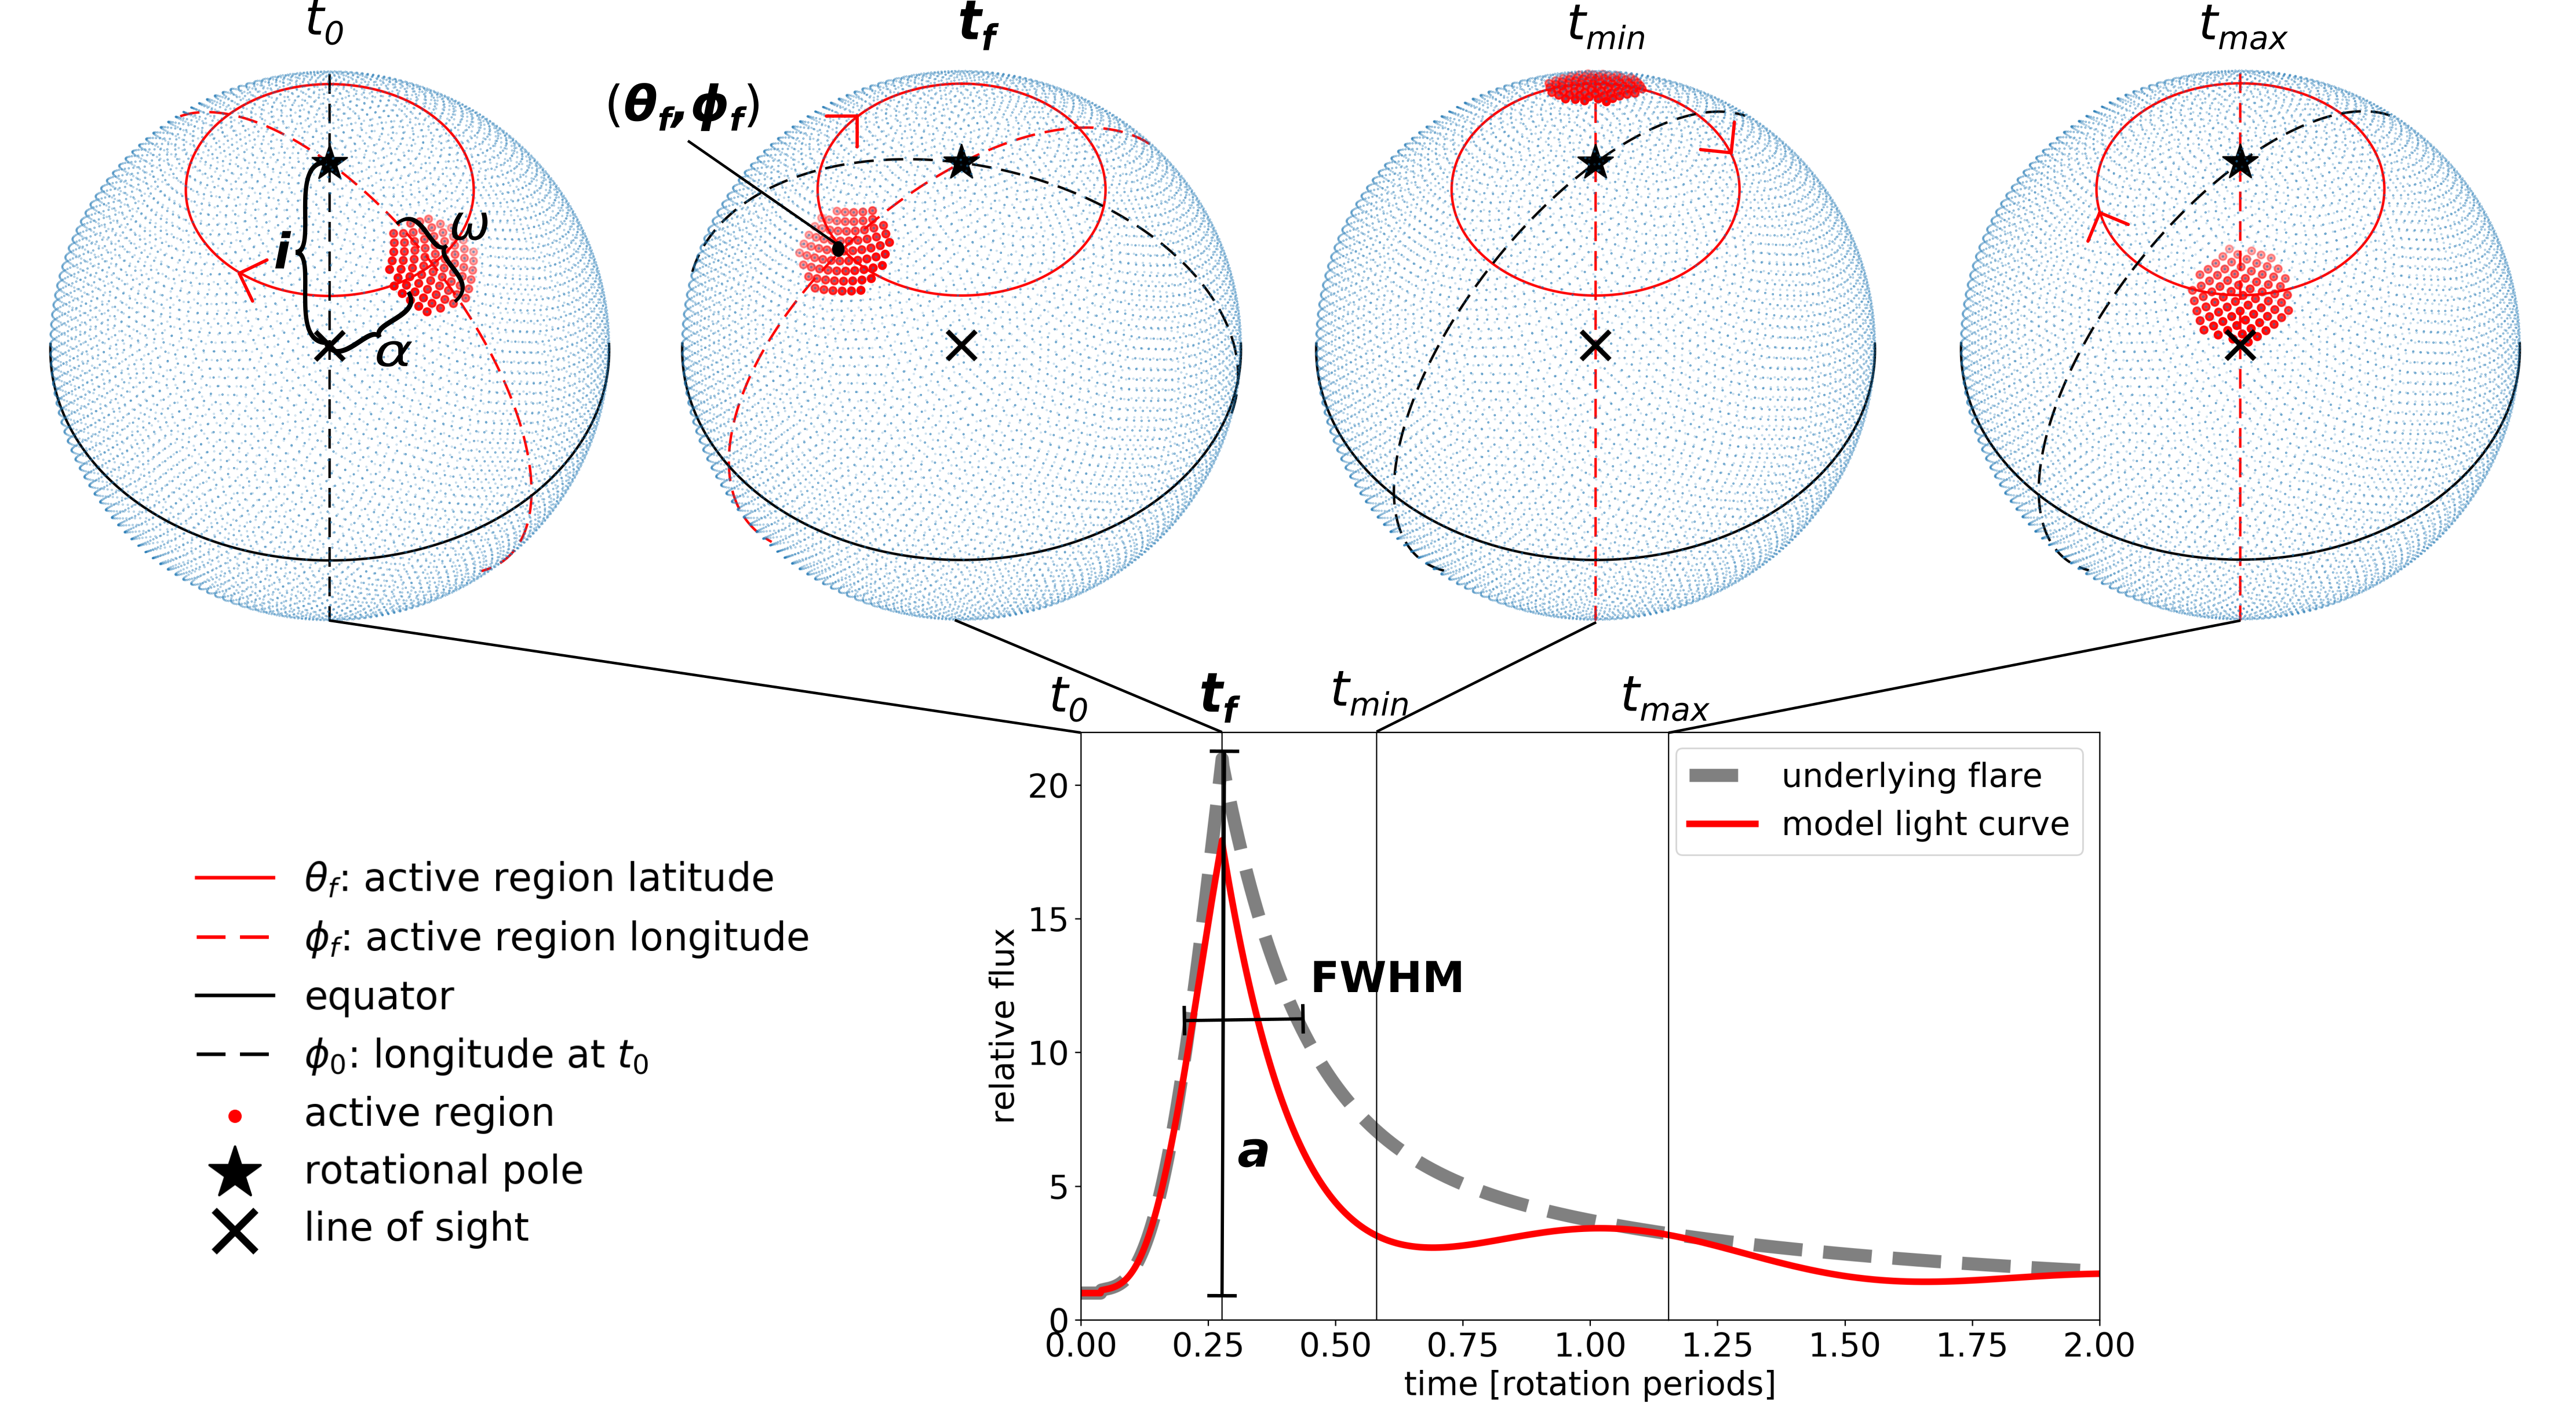
\includegraphics[width=17cm]{figures/model_illustration_annot2.png}
    \caption{The flare modulation model. From left to right, the top row shows a clockwise rotating star (blue dots) with an active region (red dots), from the start of observation at $t_0$, to the peak flare time $t_f$, and further to local minima and maxima of the rotational modulation. Note that these do not correspond to the minima and maxima of the observed flux (red line in the bottom panel). The angular distance between the rotational pole (grey cross) and the intersection of the line of sight with the center of the star $O$ (black cross) is the inclination $i$. The illustration results in the observed light curve (red) in the bottom row. The underlying flare model from~\citet{davenport2014} is shown as grey squares.}
    \label{fig:model}
\end{figure*}
% -----------------------------
%Overview of the model
Flaring regions on the Sun usually take complicated shapes that grow, shrink, brighten and dim non-uniformly with time~\citep{aschwanden2008}. The optical light curve of a flare event on a distant star hides most of this peculiar morphology. Although we expect that the flares in this study have a structure that is not resolved in Kepler and TESS data, the observed light curves can be adequately described as an empirical model flare~\citep{davenport2014} that is modulated by rotation.
%However, the FCUFRs' rapid rotation magnifies the geometric modulation that is caused by the flaring region's moving in and out of view.
\\
We designed a simple model with six parameters that were fit simultaneously~(Fig. \ref{fig:model}). The flare peak time $t_f$, and its longitude $\phi_f$ at $t_f$ and latitude $\theta_f$ define time and location of the flare. The relative flare amplitude $a$ at $t_f$ and the full width at half the maximum flux of the flare (FWHM) determine the intrinsic shape of the light curve~\citep{davenport2014}. The last parameter is the inclination $i$ of the stellar rotation axis, which is constrained by independent observations. The geometric modulation is determined by $i$, $\theta_f$ and $\phi_f$ that we combined to give the distance of the flaring region from the limb. The model light curve was constructed in three steps:
\begin{enumerate}
    \item Determine the size $\omega/2$ of the flaring region from the flare's properties (Section \ref{ssec:flaringregion}). %, that is approximated as a spherical cap with radius $\omega/2$ on the surface of the star
    \item Split the flaring region into spatial elements $(\theta, \phi)$ to calculate the spatially resolved rotational modulation of the flare flux (Section \ref{ssec:rotationalmodulation}).
    \item Apply the modulation to the intrinsic flare light curve and sum the spatial elements to obtain the model luminosity $L_{model}$ (Section \ref{ssec:modellum}).
\end{enumerate}

\subsection{Size of the flaring region}
\label{ssec:flaringregion}
We modeled the flaring region $A$, that is the photospheric footpoint, from which the white light emission originates, as a uniformly bright spherical cap with an angular radius $\omega/2$ on the stellar surface (A1\footnote{We flag all our model assumptions with abbreviations of the form A\#.}). We assumed that the region did not migrate from its initial position at the start of the observation within the time of observation (A2). The region moved in and out of view as the star rotated so that its position relative to the line of sight of the observer determined the morphology of the obtained flare light curve.
\\
Assuming that the underlying flaring process was comparable to that of spectroscopically observed solar and stellar flares~\citep{hawley1992, kretzschmar2011}, we described the flare emission in the optical as dominated by a $T_f=10\,000$ K black body (A3), and determined the specific flare flux $F_{f,s}(T_f)$ of the region by integrating the spectral energy distribution within the TESS or the Kepler passbands~(see Section \ref{sec:props}). To simplify the calculation, we chose the pole-on view of a sphere with $A$ centered on the pole, and defined the angle between the pole and any given latitude $\theta$ as $\hat\theta=\pi/2 - \theta$. We then obtained the maximum observable flare luminosity $L_{f,max}$ by integrating the geometrically modulated $F_{f,s}(T_f)$ over $A$. The modulation is simply the cosine of the incidence angle, known as Lambert's cosine law~\citep{lambert1892}, that is equal to $\theta$ for an observer at infinite distance:
\begin{eqnarray}
    L_{f,max}&=&R^2  \displaystyle\int\int_A F_{f,s}(T_f) \cos\hat\theta \mathrm {d}A\\
    &=& R^2 F_{f,s}(T_f) \displaystyle\int_{0}^{2\pi}\mathrm{d}\phi\int_{0}^{\omega/2}\mathrm{d}\hat\theta \sin\hat\theta\cos\hat\theta\\
    &=& 2\pi R^2 F_{f,s}(T_f)\left[-\tfrac{1}{2} \cos^2\hat\theta\right]^{\omega/2}_0 \\
    &=& \pi R^2 F_{f,s}(T_f) \sin^2\tfrac{\omega}{2}
    \label{eq:Lmax1}
\end{eqnarray}
In the integration boundary, $\omega$ was the full opening angle of the cap which could take values between 0 and $\pi$. We fitted for flare parameters FWHM and $a$ in the regime where we viewed the flare at its maximum visibility, that is, viewed directly along the line of sight. The maximum observable flare flux was the product of $a$ with the quiescent stellar luminosity $L_{*}$ in the Kepler or the TESS band~(see Section \ref{sec:props}):
\begin{equation}
L_{f,max} = a \cdot L_{*},
\label{eq:Lmax2}
\end{equation}
Combining Eqn.~\ref{eq:Lmax1} and~\ref{eq:Lmax2} yielded the angular radius $\omega/2$ of a circular region that produced a flare with a given amplitude $a$ and temperature $T_f$ on a star with radius $R$ and quiescent luminosity $L_{*}$:
\begin{equation}
\omega/2 = \arcsin\left(\sqrt{\dfrac{a \cdot L_{*}}{\pi R^2 F_{f,s}(T_f)}}\right)
\end{equation}
%The angular radius $\omega/2$ of the active region grows with the flare amplitude.
\subsection{Rotational modulation}
\label{ssec:rotationalmodulation}
The flaring region with radius $\omega/2$ centered on $(\theta_{f},\phi_{f})$ was represented by an ensemble of $N$ evenly distributed spatial elements. It was assumed to emit uniformly (A1), so each spatial element emitted the same fraction $F_f(t)=L_f(t)/N$ of $L_f(t)$ at any given time $t$ during the flare. Before and after the flare the region emitted the average quiescent stellar flux. To model the maximum flare flux $F_f(t)$, we adopted the~\citet{davenport2014} flare model that fully describes a flare by its FWHM, amplitude $a$ and peak flux time $t_f$.
\\
The phase of the flaring region changed with rotation, but not its position on the sphere (A2). %To capture this geometric effect, we determined the distance . Accounting for the axis inclination $i$ we applied Lambert's cosine law to obtained the modulated flux.
For ease of calculation, we converted $t$ to phase in units of radian $\hat t$ using the rotation rate of the star
\begin{equation}
\hat t = \dfrac{2\pi(t - t_{0})}{P},
\end{equation}
where $t_{0}$ marked the start time of the light curve that we selected for the model fit, and $P$ was the rotation period of the star.
\\
Every spatial element emitted a modified flux $F_f(\theta,\phi,\hat t)$ of its maximum flux $F_f(\hat t)$ towards an observer at infinite distance. The modification was again given by Lambert's cosine law with incidence angle $\alpha$:
\begin{equation}
   F_f(\theta,\phi,\hat t) = F_{f}(\hat t)\,\cos\alpha(\theta,\phi,\hat t).
  % F(\theta,\phi,\hat t) &=& F_{f,s}(T_\f)  \left(\sin(\theta) \cos(i) + \cos(\theta) \sin(i) \cos(\hat t-\phi-\phi_0)\right)
 	\label{eq:lambert1}
\end{equation}
$\alpha$ was the distance from the intersection point $O$ of the line of sight with the center of the star to every spatial element ($\theta$, $\phi$)
\begin{equation}
    \alpha = \arccos\left(\sin\theta \cos i + \cos\theta \sin i \cos(\phi - \phi_0 - \hat t)\right),
    \label{eq:alpha}
\end{equation}
where $\phi_0$ was the longitude that faced the observer at $t_{0}$. Our model did not account for limb darkening or brightening effects, equivalent to the assumption that the flaring regions had no significant height in the optical (A4).% \citet{juvan2018} applied quadratic limb darkening.
\\
To determine when the spatial element was behind the limb we calculated the fractional day length $D$. Applying the spherical law of cosines to the triangle between $O$, a point on the limb at a given latitude, and the rotational pole of the star we obtained
\begin{equation}
    D = \tfrac{1}{\pi}\arccos\left(-\tan\theta \tan(\tfrac{\pi}{2}-i)\right).
    \label{eq:lambert2}
\end{equation}
Using $D$ and $\phi_0$ we defined a step function $d(\hat t)$ that was 1 when the spatial element was visible, and 0 when it was hidden:
\begin{numcases}{d(\theta,\phi,\hat t)=}
1, & if $ -D/2 < \dfrac{\phi -\phi_0 - \hat t }{ 2 \pi}  < D/2$\\
0, & else
\end{numcases}
Finally, we combined $d$ with $F_f(\theta,\phi,\hat t)$ to obtain the modulated flux of a spatial element in the flaring region
\begin{equation}
    F_{model}(\theta,\phi,\hat t) = F_f(\theta,\phi,\hat t)\,d(\theta,\phi,\hat t).
    \label{eq:lambert3}
\end{equation}
%We  map the intrinsic flaring luminosity $L_f(t)$ to $L_f(\hat t)$ and divide it by the number of spatial elements to obtain $dL_f(\hat t)/dA=F_f(\hat t)$.
\subsection{Model luminosity}
\label{ssec:modellum}
Finally, we calculated the model luminosity $L_{model}$ as a function of $\hat t$ by summing up all spatial elements. For $N\to\infty$, $L_{model}$ became the surface integral over the flaring region $A$:

\begin{equation}
    L_{model}(\hat t) = \displaystyle\int\int_AF_{model}(\theta,\phi,\hat t)\,\mathrm{d}A
              %        &=& R^2\displaystyle\int\int F(\theta,\phi,\hat t)d(\theta,\phi,\hat t)\cos(\theta)\mathrm{d}\theta\mathrm{d}\phi\\
    \label{eq:Lmodel}
\end{equation}
The integration bounds for a circular spot could in principle be found, but we preferred the numerical approximation in the implementation that will allow us to model more complicated shapes in the future and spared us some hideous integrals.
\citet{juvan2018} used a similar approach to model starspots and transits.
\subsection{Fitting the model to the data}
\label{ssec:fittingmodeltodata}
We removed the dominating starspot modulation with a simple sine fit with the dominating period obtained from a Lomb-Scargle periodogram~\citep{lomb1976, scargle1982}, and assumed that the star was uniform otherwise (A5).%checked periodograms, only aliases, but otherwise good fits.
We constructed a likelihood function assuming that the uncertainty in flux (\texttt{PDCSAP\_FLUX\_ERR}) was Gaussian. Our priors were uniform for all parameters but $i$, for which we adopted a Gaussian prior. Using the MCMC method~(\texttt{emcee},~\citealt{foreman_mackey2013}) we determined the posterior distributions of the intrinsic flare properties FWHM, $t_f$, and $a$; the properties of the flaring region, $\theta_f$ and $\phi_f$; and an updated distribution of the inclination $i$ of the star's rotation axis.
% More caveats perhaps not relevant
%Also did not account for gravitational darkening that stems from rotation and could have an effect on the contrast of the flare, and alter the geometric setup from a sphere to an ellipsoid~\citep{sengupta2010}
\subsection{A3 -  10 000 K BB}
\citet{kowalski2013} found a peak blckbody temperature of 10 000 K to be constant for different flare amplitude over two orders of magnitude
\section{Results}
% --------------------------------------------------------
\begin{figure*}
	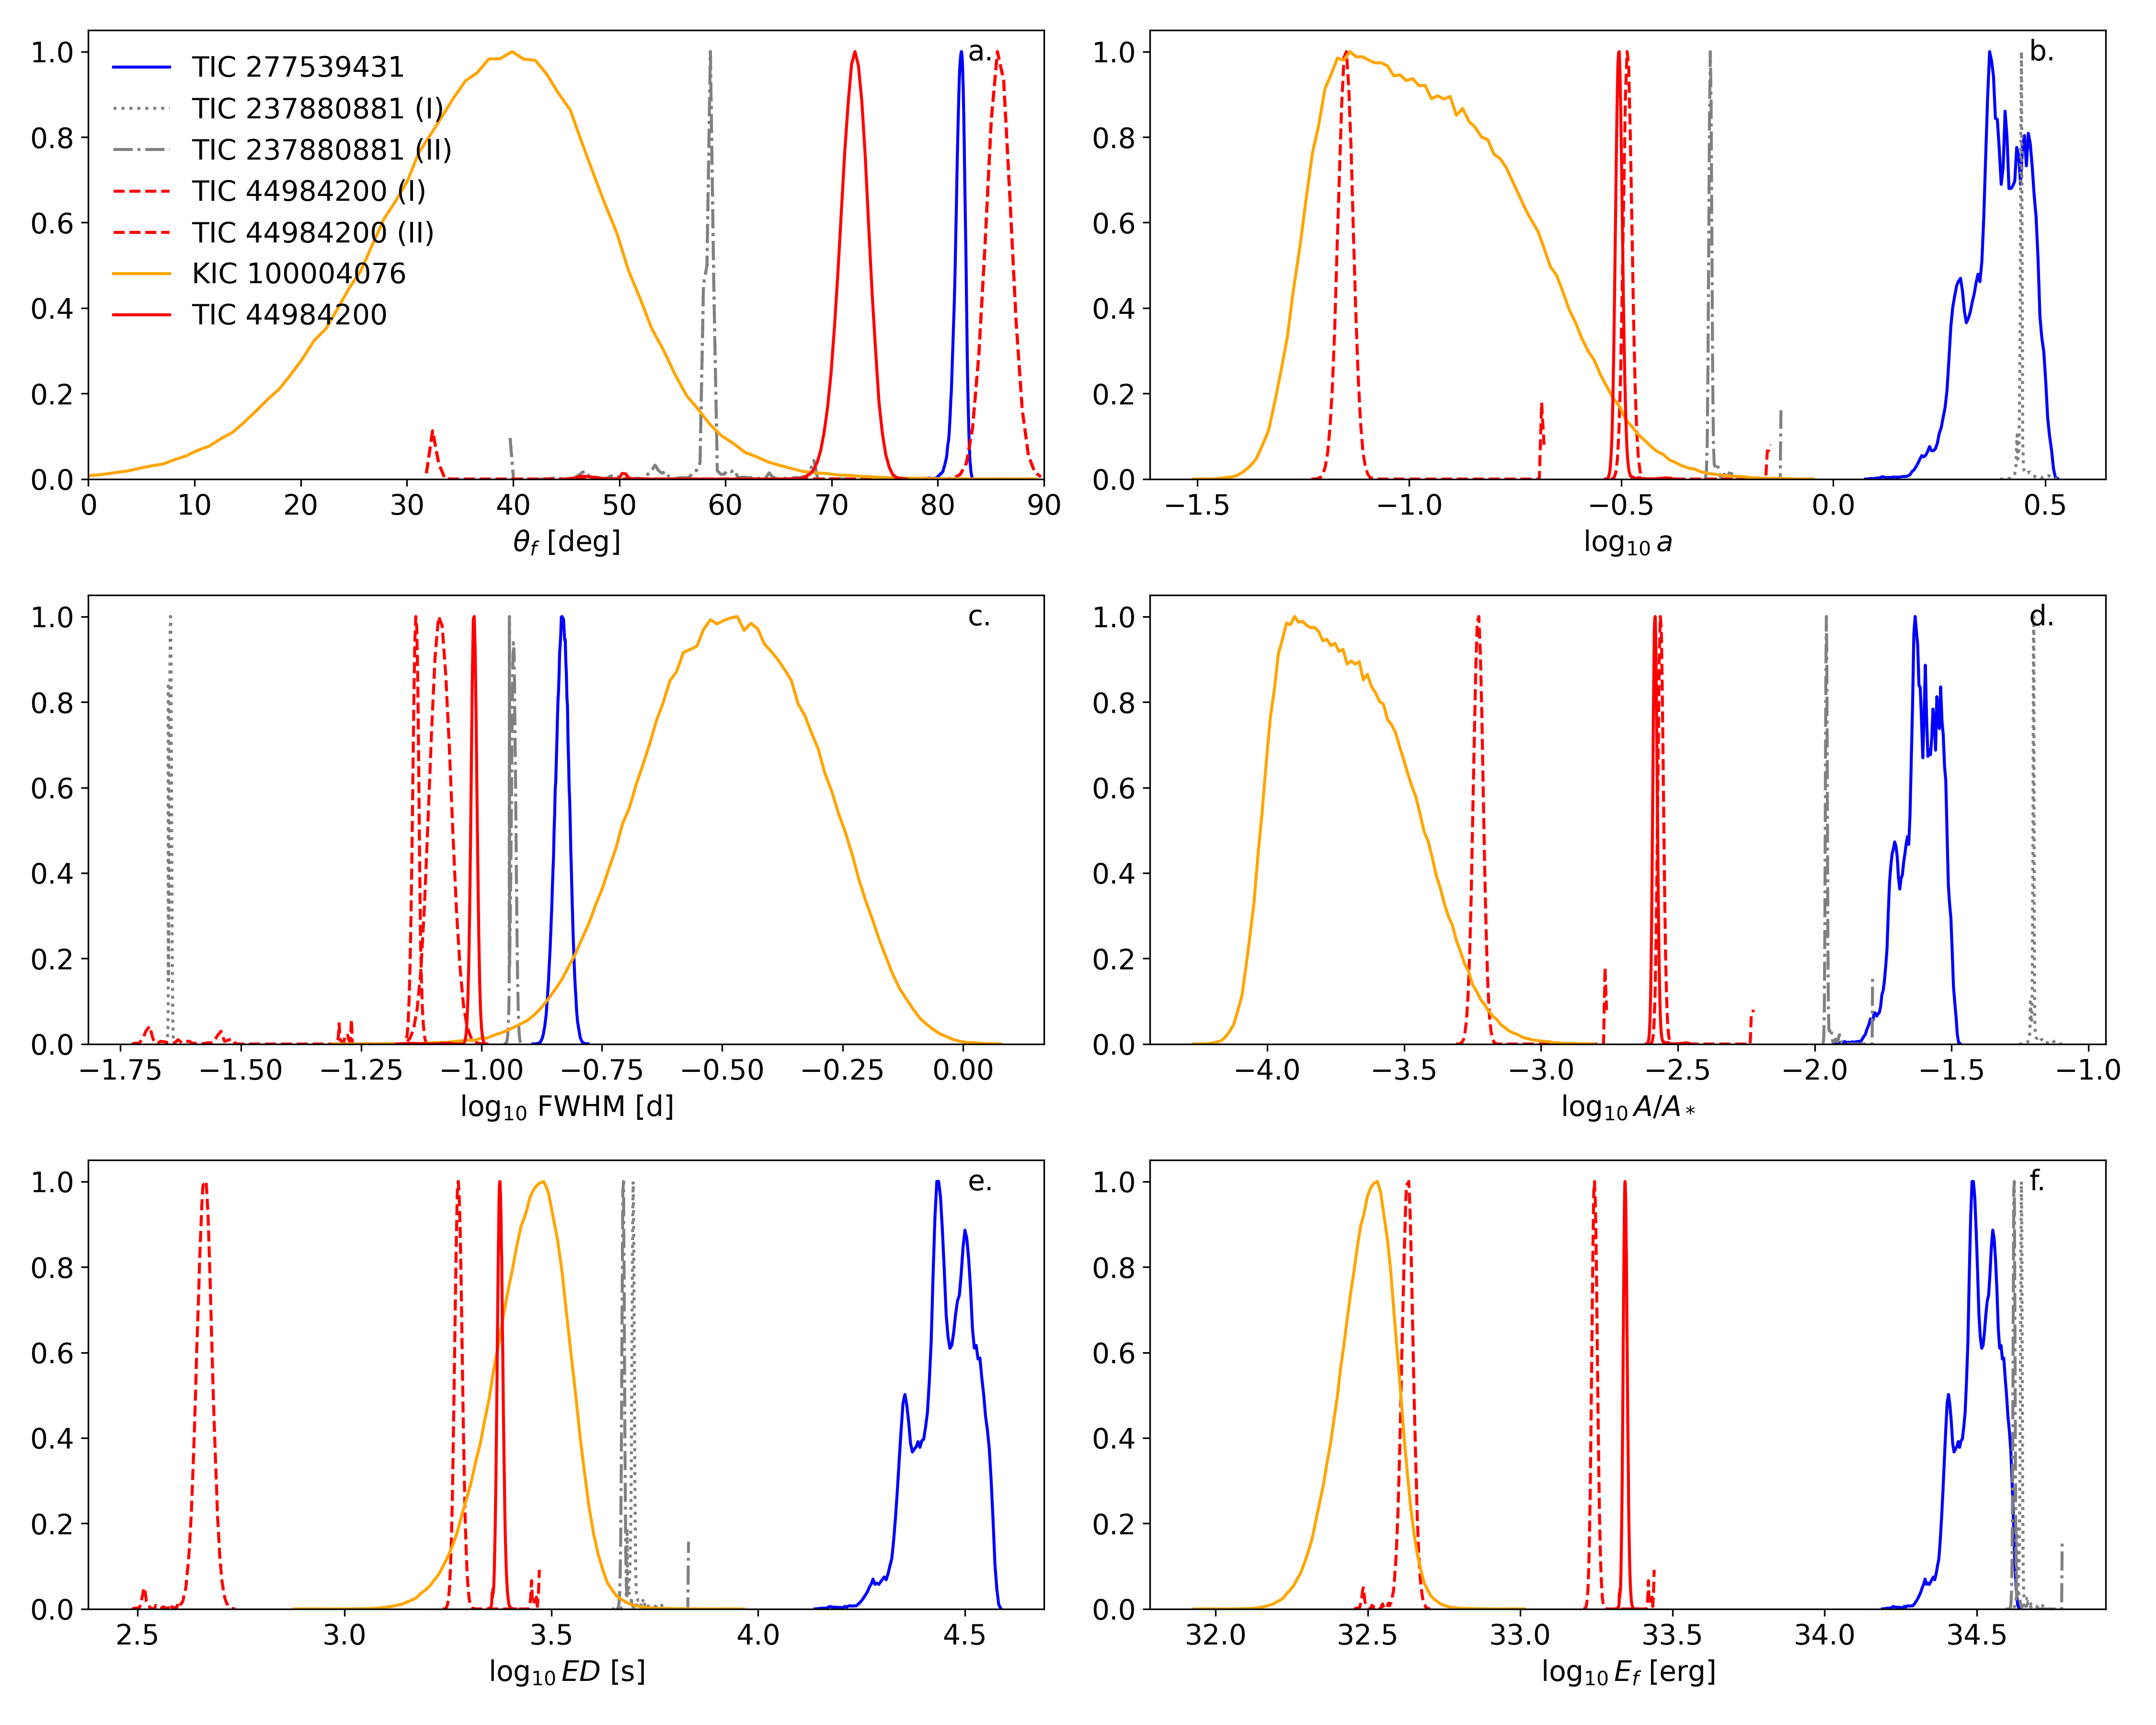
\includegraphics[width=\hsize]{figures/12_08_2020_posteriors.png}
    \caption{Posterior distributions of model fits to multiperiod flares. a. Flaring region latitude. b. Logarithm of relative flare amplitude of the underlying flare. c. Logarithm of FWHM of underlying flare. d. Logarithm of size of the flaring region as a fraction of the total stellar surface $A$. e. Logarithm of equivalent duration of underlying flare. f. Logarithm of energy released in the course of the underlying flare in Kepler or TESS band.}
    \label{fig:posteriors}
\end{figure*}

We fitted our model with either one or two flares occurring on a single active region. We did not attempt to fit multiple active regions. The probability of two large flares occurring within a very short period is very low if we assume that flare times follow a Poission process in time, like it does on the Sun and most flaring stars. \textbf{Calculate the actual probability using the FFD analysis.} Consequently, the flares are likely to be sympathetic, that is, emerging from the same active region.

\label{sec:results}

\begin{table*}
\centering
\caption{Fitted properties of multi-period flares.}
\label{tab:stars}
\begin{tabular}{lccccccccr}
\hline\hline
             ID &                              $t_0$ (BJD) &      $E_{f}$ (erg)$\cdot 10^{33}$ &                          $ED$ (s) &                             $A/A_*$ &                     $\phi_0$ (deg) &                               $a$ &                      $i$ (deg) &                              FWHM (d) &                 $\theta_f$ (deg) \\
\hline
      277539431 &    $1641.84461\left(^{123}_{176}\right)$ &  $32.02\left(^{545}_{535}\right)$ &  $28430\left(^{484}_{475}\right)$ &  $0.02448\left(^{434}_{421}\right)$ &     $240.7\left(^{26}_{32}\right)$ &  $2.464\left(^{423}_{415}\right)$ &  $86.6\left(^{20}_{22}\right)$ &    $0.07355\left(^{233}_{241}\right)$ &      $82.1\left(^{4}_{5}\right)$ \\
  237880881 (I) &        $1331.66387\left(^{2}_{2}\right)$ &    $44.24\left(^{39}_{43}\right)$ &       $4988\left(^{4}_{5}\right)$ &    $0.06300\left(^{32}_{49}\right)$ &       $158.8\left(^{1}_{0}\right)$ &    $2.776\left(^{13}_{20}\right)$ &    $22.0\left(^{5}_{8}\right)$ &        $0.01130\left(^{6}_{6}\right)$ &      $58.5\left(^{3}_{6}\right)$ \\
 237880881 (II) &      $1331.82654\left(^{14}_{15}\right)$ &    $41.91\left(^{42}_{32}\right)$ &       $4725\left(^{5}_{4}\right)$ &     $0.01104\left(^{12}_{9}\right)$ &       $158.8\left(^{1}_{0}\right)$ &      $0.514\left(^{5}_{4}\right)$ &    $22.0\left(^{5}_{8}\right)$ &      $0.05826\left(^{61}_{64}\right)$ &      $58.5\left(^{3}_{6}\right)$ \\
       44984200 &      $1588.02563\left(^{17}_{17}\right)$ &       $2.21\left(^{4}_{3}\right)$ &       $2378\left(^{4}_{4}\right)$ &      $0.00261\left(^{5}_{5}\right)$ &     $430.4\left(^{29}_{31}\right)$ &      $0.312\left(^{6}_{6}\right)$ &  $33.1\left(^{16}_{16}\right)$ &      $0.04823\left(^{67}_{65}\right)$ &    $72.1\left(^{13}_{14}\right)$ \\
   44984200 (I) &      $1588.02191\left(^{16}_{17}\right)$ &       $1.76\left(^{4}_{4}\right)$ &       $1888\left(^{4}_{4}\right)$ &      $0.00274\left(^{7}_{6}\right)$ &   $190.2\left(^{134}_{123}\right)$ &      $0.328\left(^{8}_{7}\right)$ &  $33.0\left(^{16}_{17}\right)$ &      $0.03649\left(^{52}_{58}\right)$ &    $85.7\left(^{12}_{13}\right)$ \\
  44984200 (II) &      $1588.12528\left(^{94}_{69}\right)$ &       $0.43\left(^{2}_{2}\right)$ &        $458\left(^{2}_{2}\right)$ &      $0.00059\left(^{3}_{2}\right)$ &   $190.2\left(^{134}_{123}\right)$ &      $0.071\left(^{3}_{3}\right)$ &  $33.0\left(^{16}_{17}\right)$ &    $0.04096\left(^{216}_{210}\right)$ &    $85.7\left(^{12}_{13}\right)$ \\
      100004076 &  $1358.63262\left(^{5918}_{5144}\right)$ &       $0.33\left(^{7}_{7}\right)$ &     $2957\left(^{61}_{59}\right)$ &     $0.00020\left(^{15}_{8}\right)$ &  $-138.5\left(^{607}_{489}\right)$ &    $0.114\left(^{88}_{43}\right)$ &  $57.8\left(^{65}_{65}\right)$ &  $0.16332\left(^{8395}_{5569}\right)$ &  $46.0\left(^{116}_{137}\right)$ \\
\hline

\end{tabular}

Values in parentheses are the differences to the $84$th (upper) and $16$th (lower) percentiles in digits counted backwards from the displayed value ($50$th percentile).
\end{table*}
We fitted the flare modulation model to the data. Our results are summarized in Table \ref{tab:results}.

\subsection{\FC}

% --------------------------------------------------------
\begin{figure}
	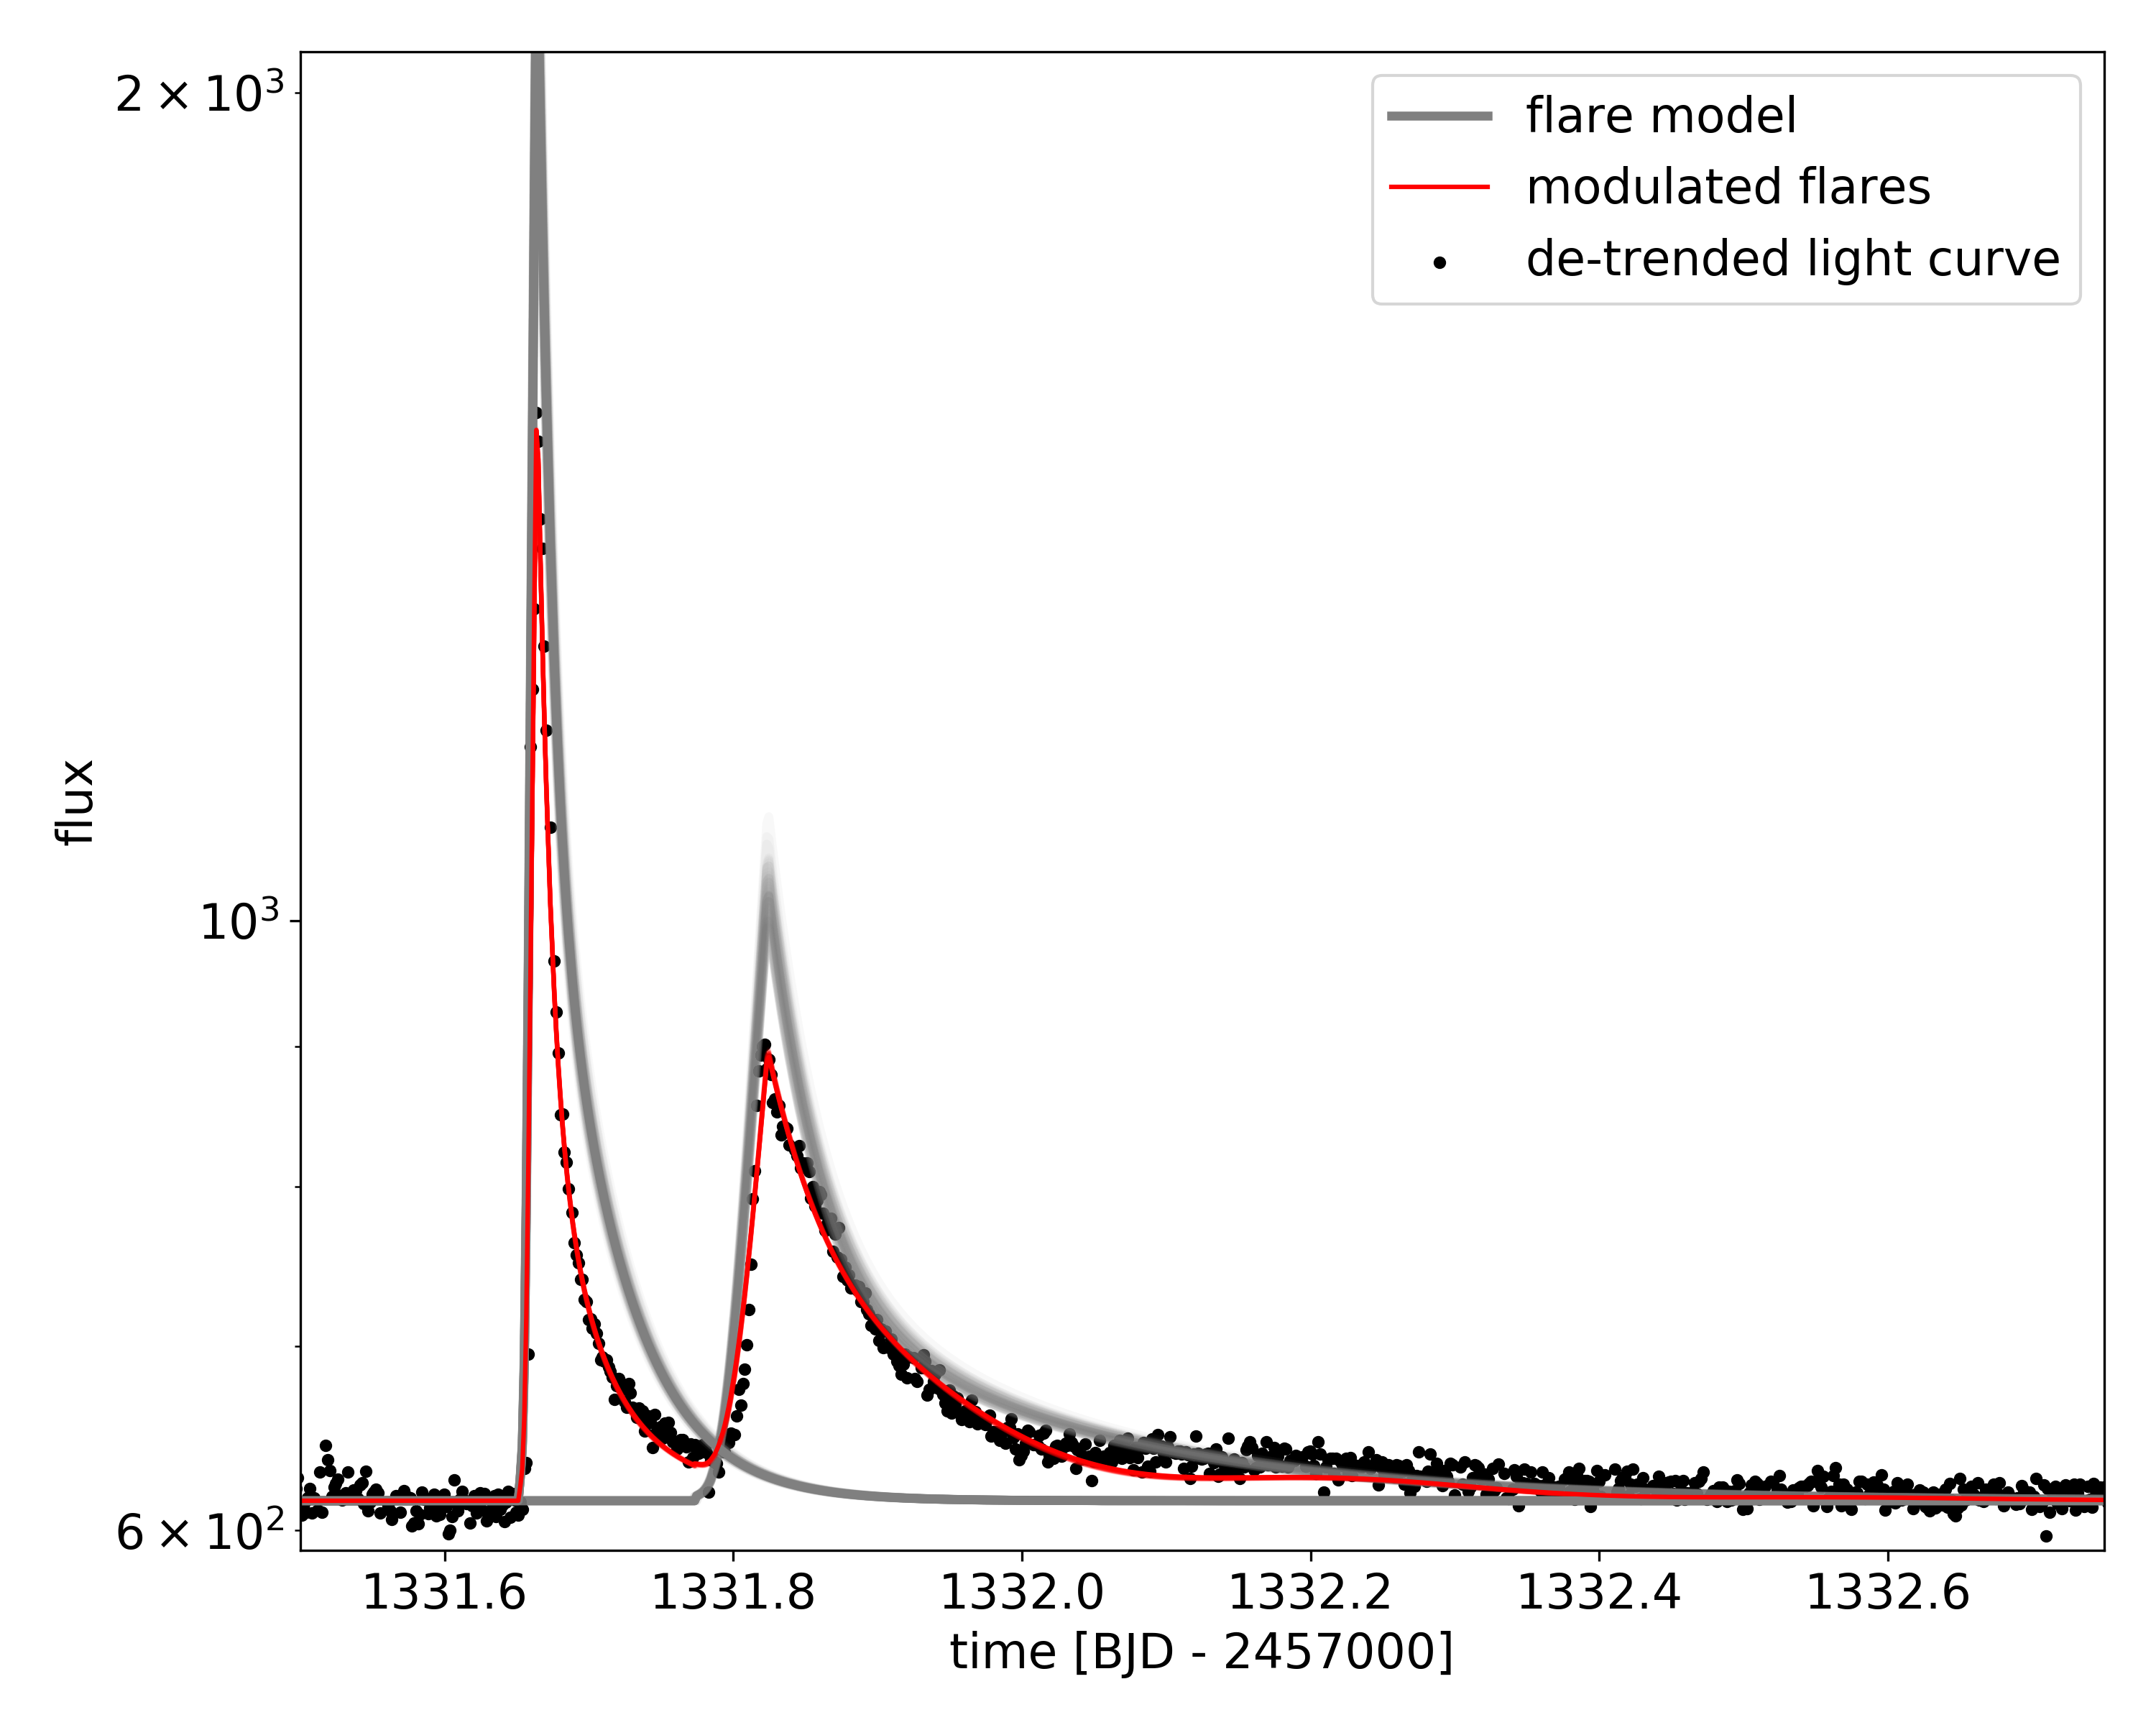
\includegraphics[width=\columnwidth]{figures/23_12_2019_13_28_TIC237880881_flarefit_50retrievals.png}
    \caption{Double-flare fit to \FC, assuming that both flares originate from the same active region ($\theta_f$ is the same for both flares).}
    \label{fig:fit\FC}
\end{figure}
% --------------------------------------------------------
This light curve contains two overlapping flares. Since the first flare's gradual decay adds to the overall flux in the second flare we fitted both flares simultaneously.
\\
\citet{gizis2017b} discussed the possibility of sympathetic flaring in ultracool dwarfs that is triggered by fast mode MHD waves excited by the first flare that propagates across an inhomogeneous corona to trigger a second flare, as is the case on the Sun~\citep{uchida1968}. They concluded that such flares are characterized by a time separation between flares that is inconsistent with a Poisson process, and a lower amplitude second flare. The flares in \FC have both traits. However, the flares are separated by 3-4 hours which suggests travel speeds of less than 40 km/s pole to pole, lower than the lowest observed speeds on the Sun at 200 km/s. Futhermore, on the Sun these waves are driven by erupting CMEs which are suppressed by strong dipolar large scale fields of mid-M dwarfs~\citep{alvaradogomez2018} (but in a 75G large scale field >3e32 erg flares can overcome the suppression and erupt anyways.)
\subsection{\FB}
The flare on \FB was visible for almost five rotation periods. While the flux appeared modulated, the flaring region never fully rotated out of view, indicating a latitude significantly above the inclination value of 33 degrees. We fitted the single flare model (Fig. \ref{fig:fit\FB}), and a model with two flares that occur on a single active region (Fig.~\ref{fig:fit2\FB}). Both fits indicated that the flare(s) occurred at high latitudes, at $72$ and $86$ degrees for the one- and two-flare solutions, respectively. However, the difference in latitudes is inconsistent with the uncertainties for each solution~(Fig.~\ref{fig:posteriors}). We suspect that the flare was complex, with multiple superimposed flares that mostly affected the fast decay phase. The gradual decay phase was well fit by the one-flare solution. It is also possible that the secondary flare(s) occurred at latitudes other than the main flare, or that our circular model of flaring region geometry was an oversimplification. \textbf{But the former should be unlikely, or? Give propbability from FFD analysis of non-sympathetic flares overlapping like this.}
\begin{figure}
	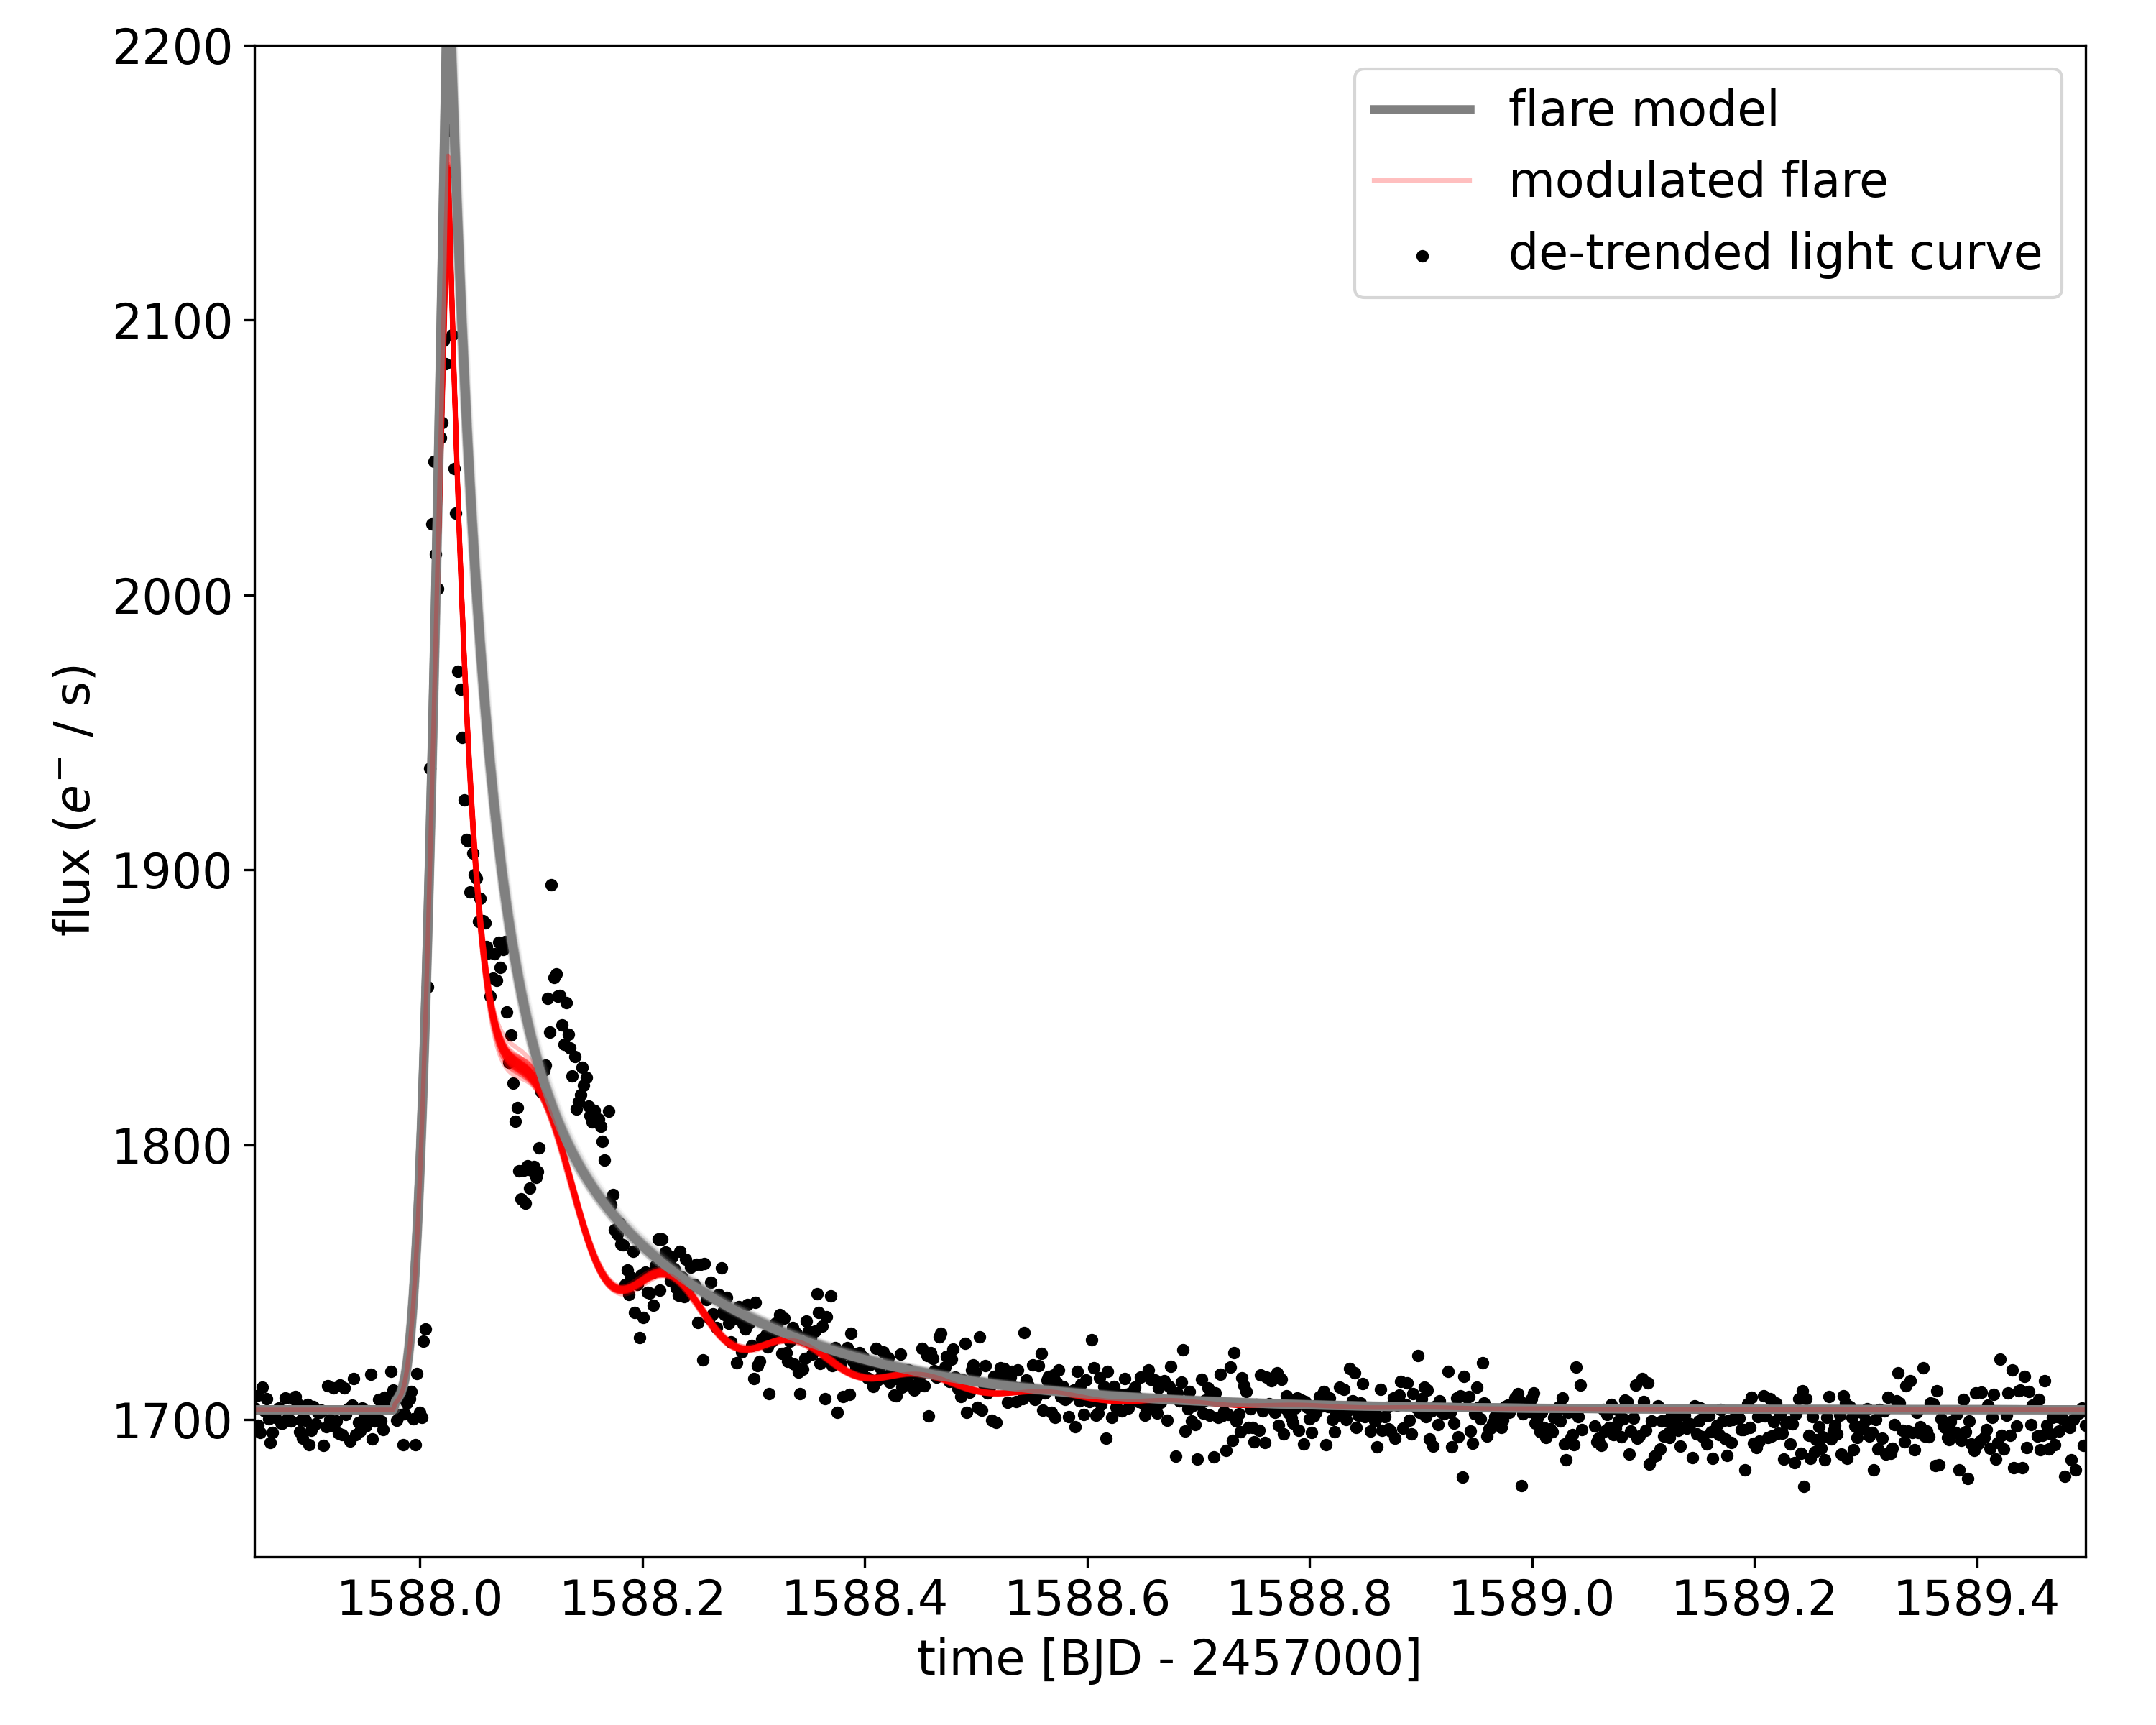
\includegraphics[width=\columnwidth]{figures/02_08_2020_17_44_TIC44984200_flarefit_50retrievals.png}
    \caption{Single-flare fit to \FB.}
    \label{fig:fit\FB}
\end{figure}
\begin{figure}
	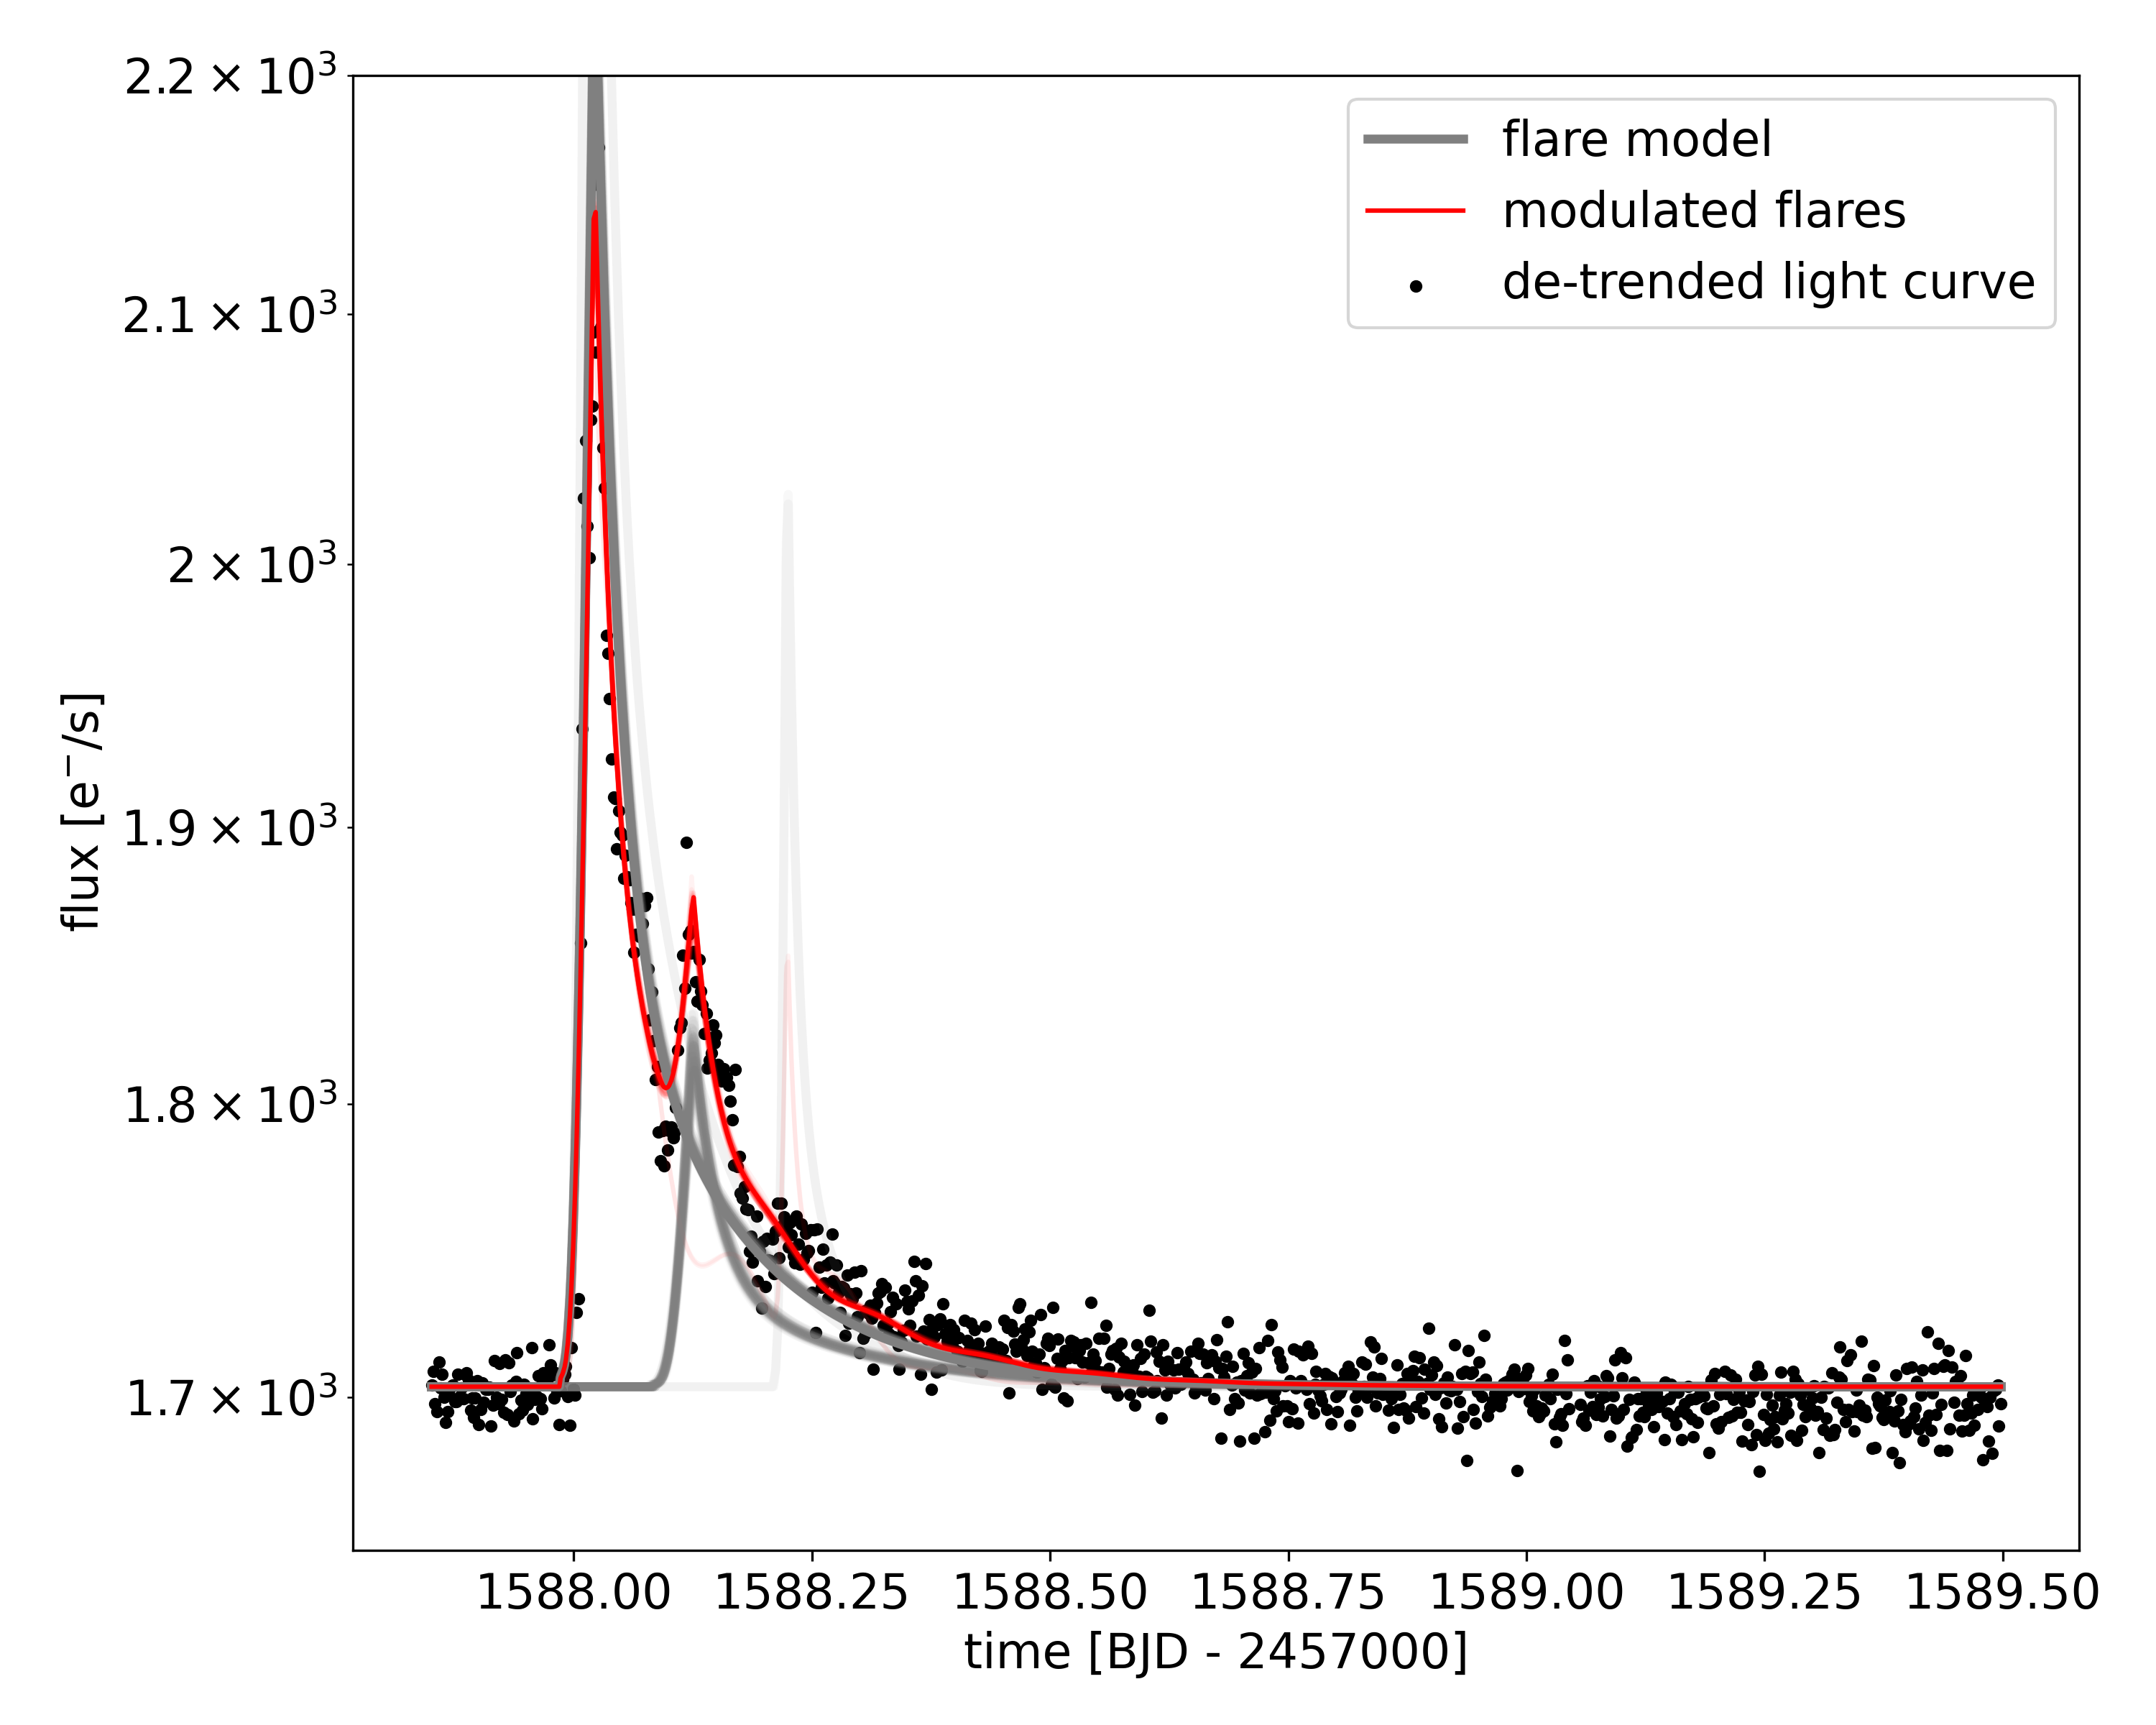
\includegraphics[width=\columnwidth]{figures/04_08_2020_13_40_TIC44984200_flarefit_50retrievals.png}
    \caption{Two-flare fit to \FB.}
    \label{fig:fit2\FB}
\end{figure}
\subsection{\FA}
% TIC 277
The flare on \FA lasted for more than three rotation periods. The flare flux disappeared and reappeared \FA at least two times after the main peak, but only briefly and smoothly, suggesting an active region latitude somewhat below the inclination value of 87 degrees. Indeed, the signal was best fit by a single flare that occurred at $82$ degree latitude. The inferred area is large, covering about $2.5\%$ of the stellar surface, consistent with the high inclination of the star and the smooth modulation of the light curve~(Fig. \ref{fig:fit\FA}). Our model fit implies that the underlying flare had an amplitude of $\sim 2.5$, and that the peak occurred on the far side of the star. The flaring region then rotated into view during the fast decay phase, and the gradual decay emission was still observable two rotations later. The inferred flare energy released in the TESS band was $3.2\cdot 10^{34}$ erg

% --------------------------------------------------------
\begin{figure}
	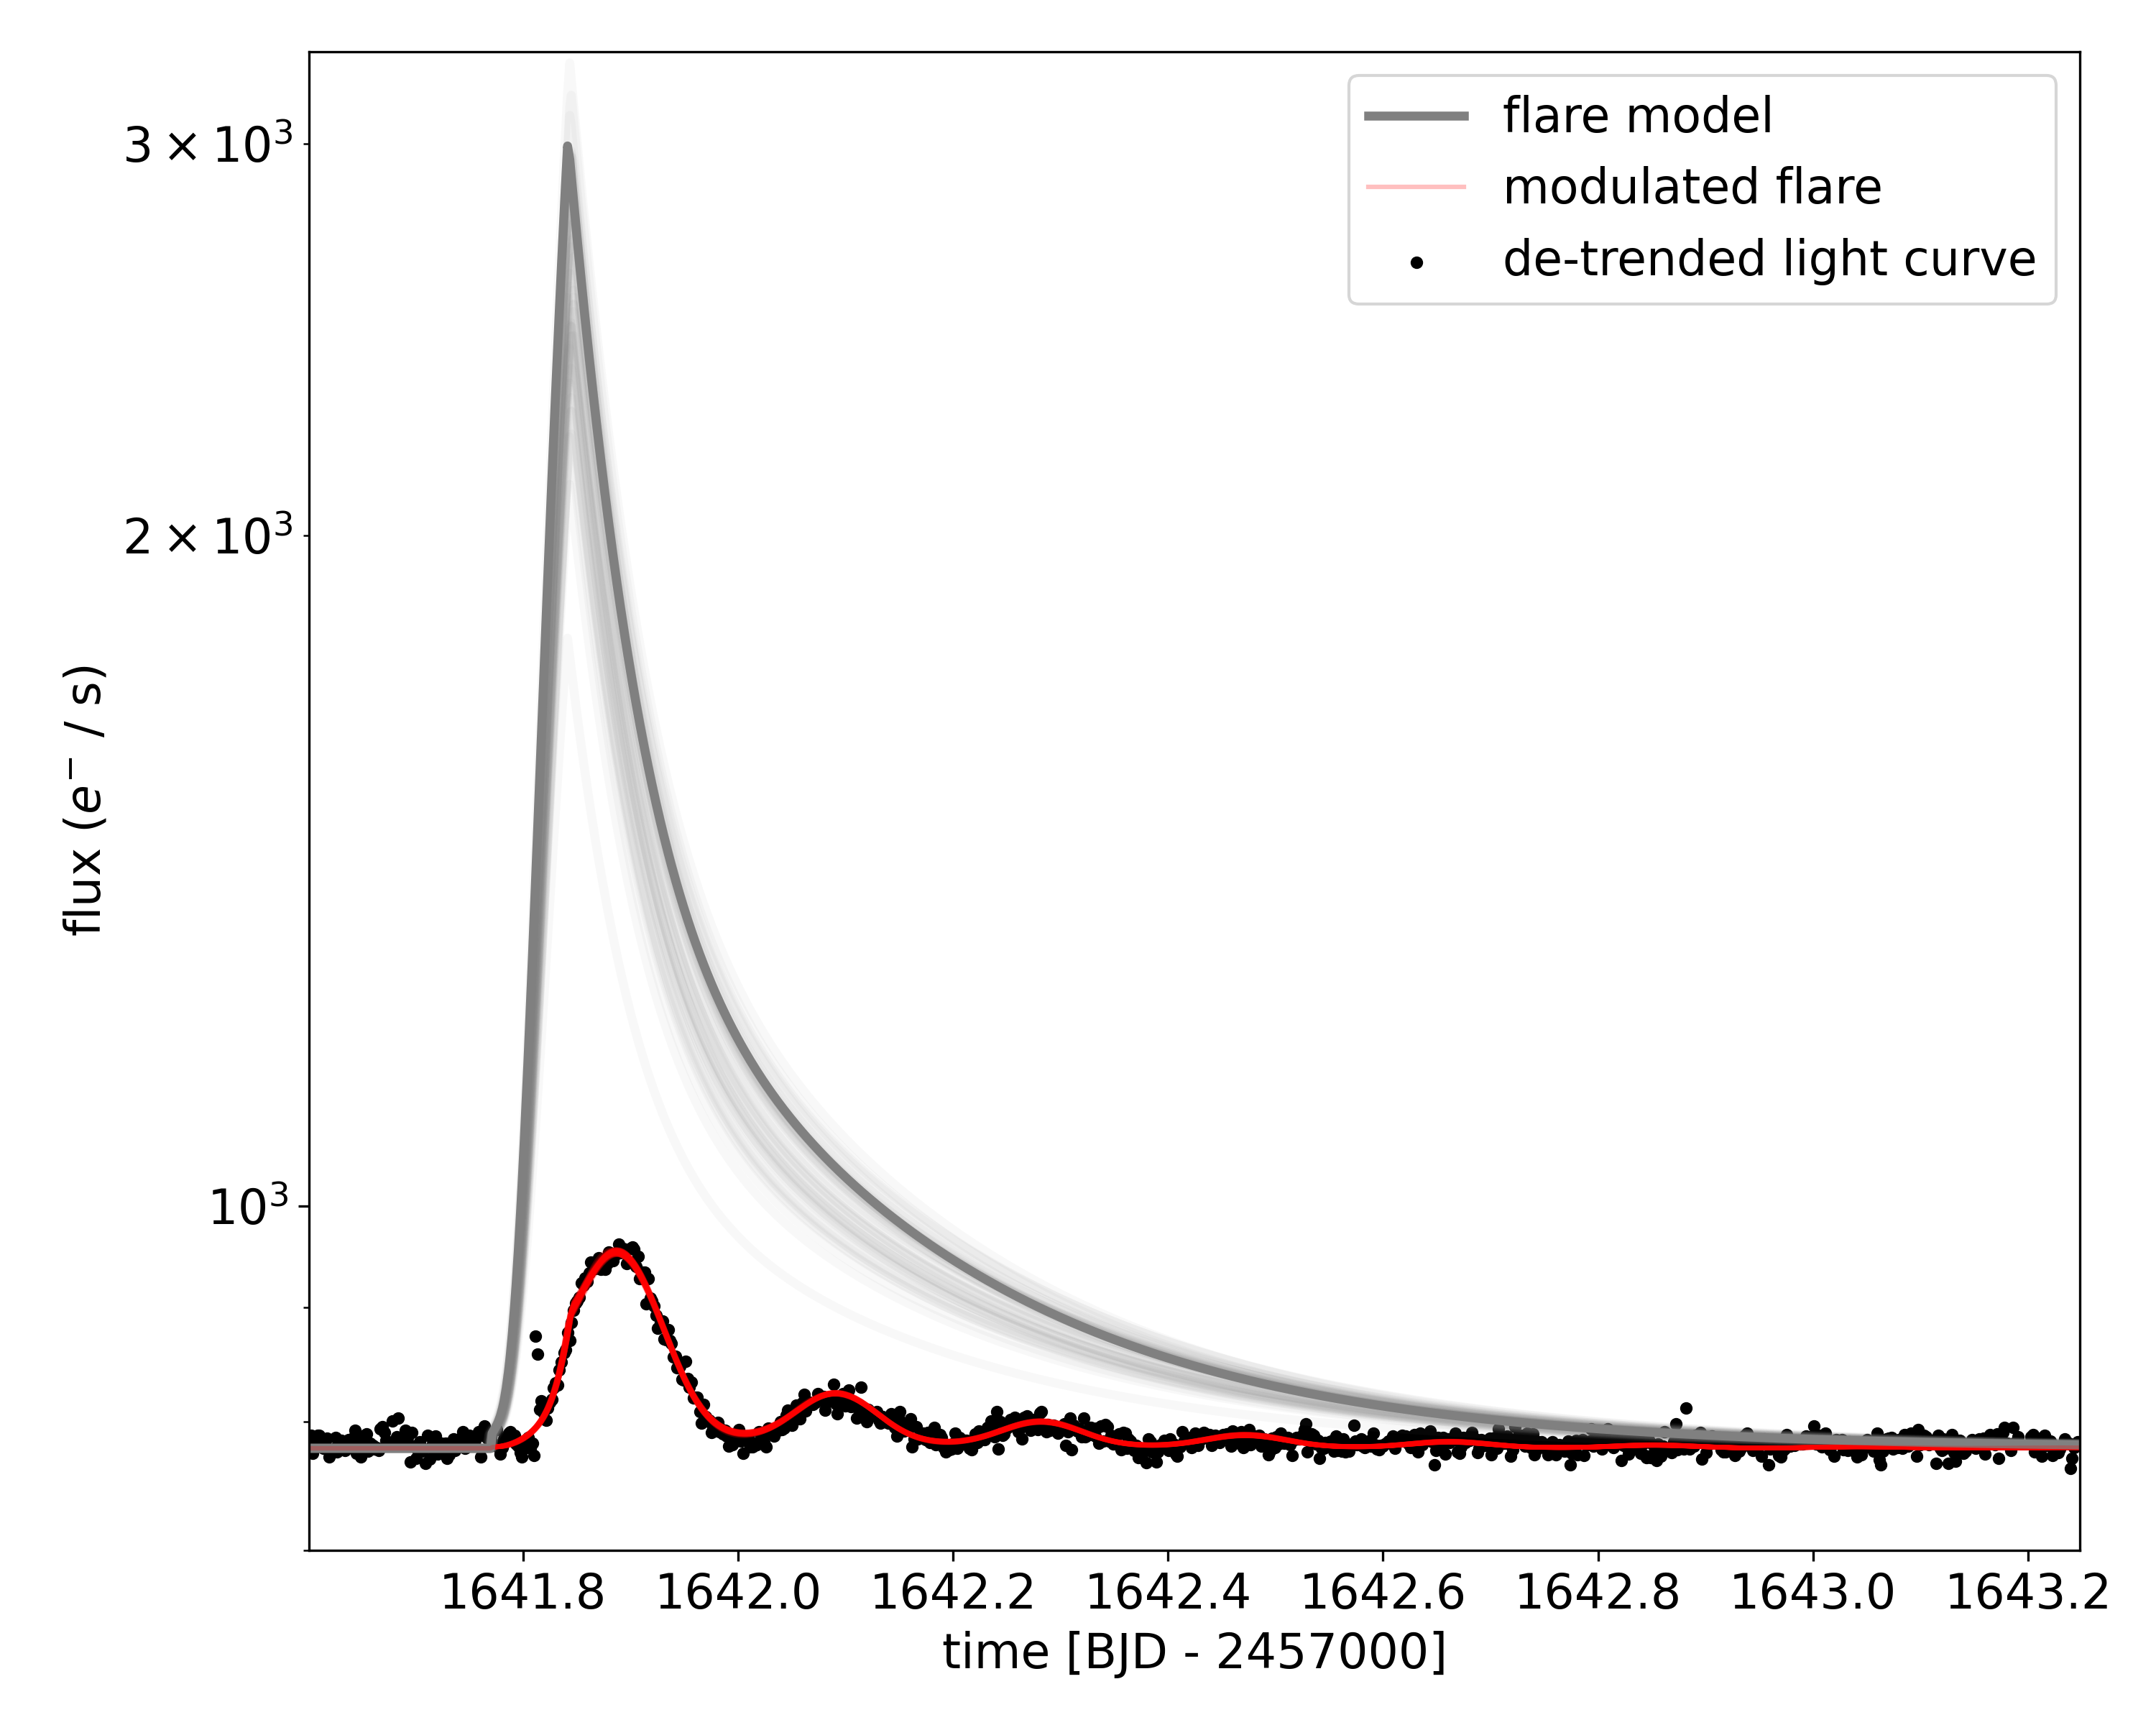
\includegraphics[width=\columnwidth]{figures/08_07_2020_11_48_TIC277539431_flarefit_50retrievals.png}
    \caption{Flare fit to \FA.}
    \label{fig:fit\FA}
\end{figure}
% --------------------------------------------------------



\subsection{\FE}
% --------------------------------------------------------
\begin{figure}
	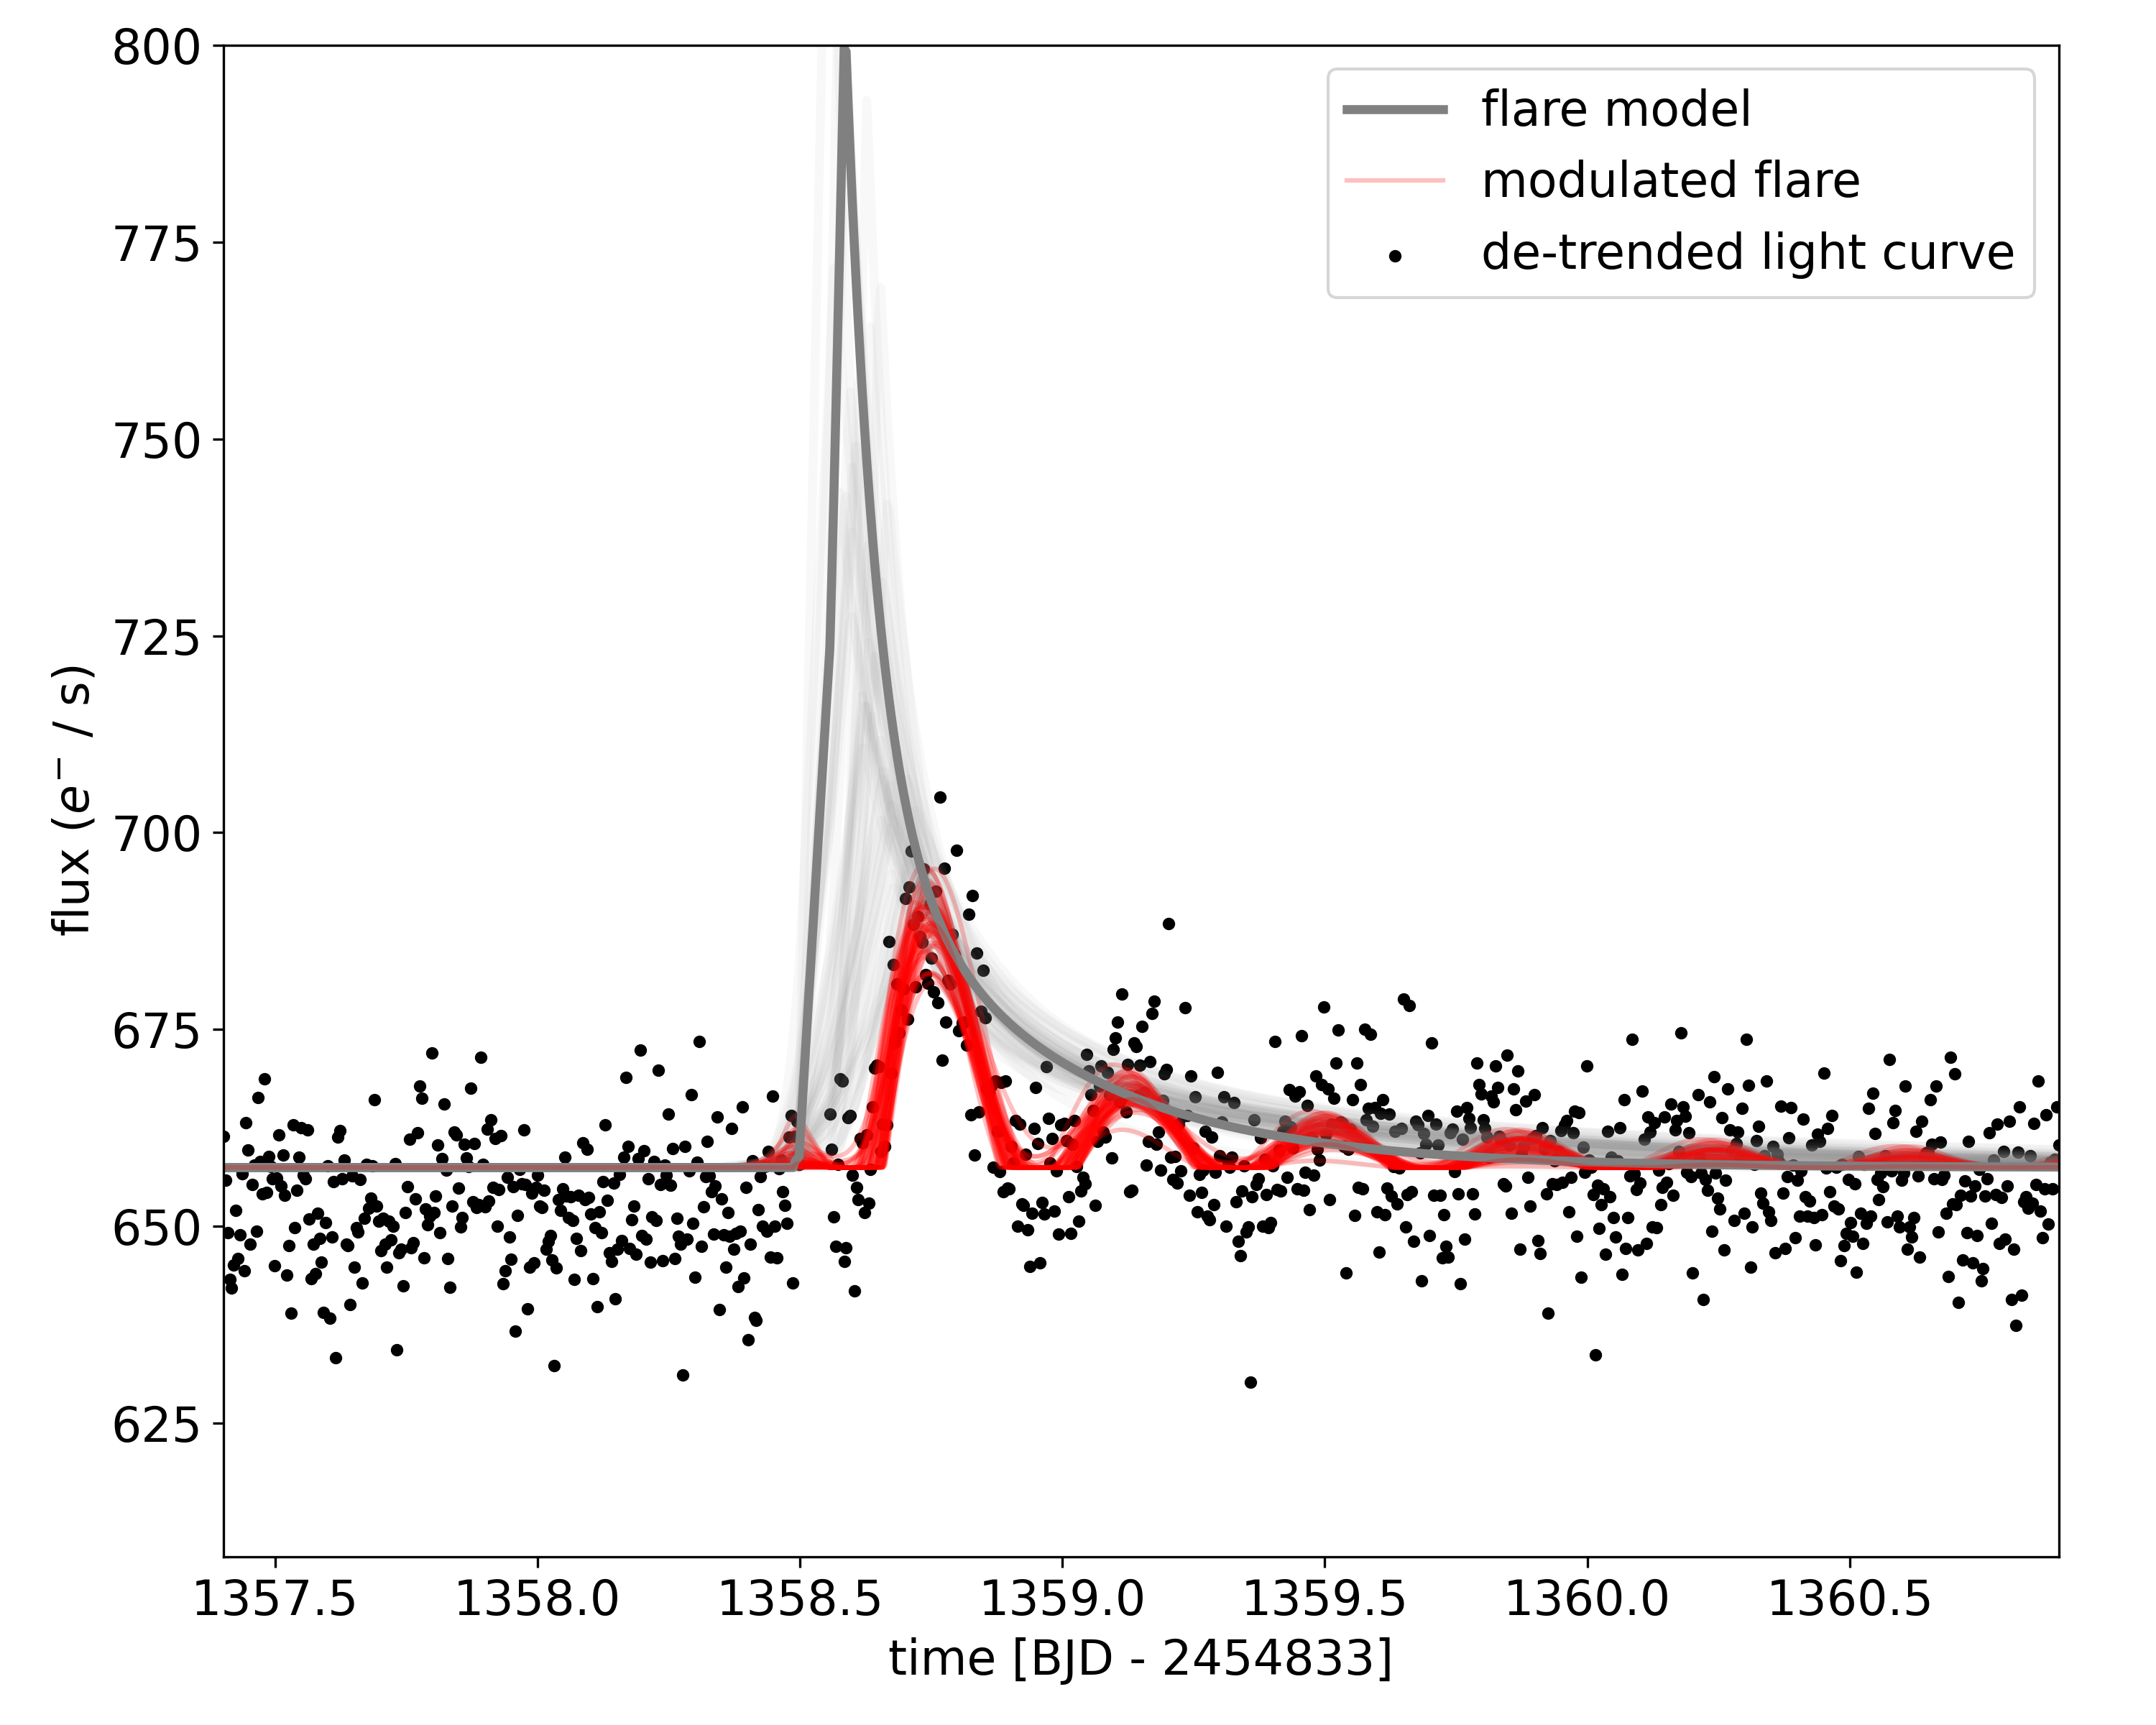
\includegraphics[width=\columnwidth]{figures/04_08_2020_14_26_KIC100004076_flarefit_50retrievals.png}
    \caption{Flare fit to \FE.}
    \label{fig:fit\FE}
\end{figure}
% --------------------------------------------------------
We recovered the extremely stable 8.9 h periodicity, measured in five Kepler quarters from \citep{gizis2013}. The flare on \FE appeared impulsive and short, but the excess flux observed during the rotation period after the impulsive rise and decay in excess of the rotational modulation was a hint that the flare could in fact have been much stronger and lasted multiple periods. However, the MCMC chain did not converge, and ended in an extreme underlying flare~(Fig. \textbf{TODO}). We therefore fitted the alternative model in which the short first flare is a precursor to the multiperiod flares, and not part of the modulated event of which we in fact miss the peak~(\ref{fig:fit\FE}).

\\
% Still, \FE had the most gradual solution, that is, the small ratio of amplitude to FWHM. discuss difference between TESS and Kepler band 
\\
\textbf{Which one would be more likely given its properties, like amplitude-duration ratio, total energy etc.?}

\subsection{Active region radii}
We converted angular radii $\omega/2$ of the flaring regions from our model fits to fraction of stellar surface $A/A_*$~(Table~\ref{tab:stars}). We find values between $0.02\%$ for the smallest flare on \FE, and more than $6\%$ for \FC (I). The amplitudes of our flares were between $0.08$ and $2.8$. Large mid-M dwarf flares with detected peaks in multiwavelength observations have flare surface areas of $0.0015\%–0.11\%$~for flares with U band amplitudes between .5 and 200~\citep{kowalski2013}. On CN Leo, the fractional area for a flare that increased the flux in the UVES red band ($4200-10000\AA$) by a factor of 40, and $550$ in the blue band ($3000-5000\AA$) was estimated at about $0.1\%$ assuming $T_{BB}=10 000$ K~\citep{fuhrmeister2008}. An extremely large flare on an M8 dwarf that temporarily increased the brightness by almost a factor 4000 in V band had estimated $A/A_*$ ranging from $3.25\%$ to $8\%$~assuming $T_{BB}$ between 10 000 K and 16 000 K~\citep{schmidt2014}\footnote{Note that the filling factor, that is the fractional area of the projected visible hemisphere is higher than $A/A_*$ by a factor of four.}.
\\
The area $A$ from which the blackbody emission originates increases during the rise phase, and is approximately constant during the decay phase. This echoes the blackbody temperature $T_{BB}$, so that and $A$ are better fit simultaneously~\citep{kowalski2013}. In this study, we assumed 10 000 K for all flares, and calculated an active region size that remains constant throughout of the flare.
%---------------------------------------------------------------------
\section{Discussion}
\label{sec:discussion}

\subsection{Do flares in FCUFRs occur at the poles?}
Our results suggest that large gradual flares on stars with a large dominating spot prefer to occur at high latitudes. Potentially, the occurrence of such flares and the presence of such spots are physically related.

Given the small number of such flares, it could also be a selection effect. If flares on FCUFRs occur at all latitudes, it could just be that detectability of multiperiod flares is lower for low-latitude flares. Assuming that $i$ is uniformly distributed we find low detectability at the equator at low inclinations if the primary peak is less pronounced, and low detectability at high inclinations if the secondary peak is confused for an independent event because the the secondary peak is separated by a full half period from the primary peak. On the other hand, low detectability at the pole is found at high inclination because the primary peak height is geometrically reduced, and at low inclination because the secondary peak is less pronounced because the geometrical modulation declines.


Another explanation could be that flares close to the equator occur on active regions with shapes that are not modulated by rotation, as, for instance, active belt shapes at fixed latitudes. Alternatively, equatorial flares may light up the entire stellar atmosphere thereby precluding any modulation. However, we did not find any periodically modulated flares on stars without clean sinusoidal variability.

A further possibility is that TESS cannot detect low-latitude flares because they are much hotter than 10 000 K so that the TESS band cannot detect them.

It may also be that flares close to the equator are mostly much more impulsive and do not become multiperiodic. This raises the question why are polar flares more likely to be so gradual? Is this a feature of large polar spots in contrast with more evenly distributed active region as we infer for mid-M dwarfs? One way of adressing this question is to look at the distributions of flare properties on our targets. Several of them exhibit smaller and more impulsive flares in the same light curve, and also in different sectors.
\subsection{FFD analysis of FCUFR light curves}

Do the multiperiod flares fit in with the FFDs for the rest of the flare sample in each target?

The energy distributions of white light flares in ultracool dwarfs follow power laws across several orders of magnitude in flare energy~\citep{gizis2017b, paudel2018}.
%Why do we see rotational modulation in all cases but not in the flares? Possible solution: misalignment of rotational axis and magnetic dipole axis, like possibly in 	NLTT 33370 AB\citep{mclean2011}. See also ~\citep{pineda2017}
%\\
%
%\\
%When we do flare statistics, should we account for the flaring region size  and distribution of positions on the stellar surface? We are currently underestimating the flare energies because most flares are not observed on the center of the observable hemisphere of the star.
%\\
%Can our findings be explained by quasi-periodic pulsations (QPPs), that are a common feature of solar flares in a variety of wavelengths~\citep{pugh2016}, instead?
%QPPs were observed during superflares on solar-type and low-mass stars, for istance on YZ CMi (M4.5e) with a period of 32 minutes~\citep{anfinogentov2013}, and on KIC 9655129 (K1.5V eclipsing binary) with two periods, 78 and 32 min~\citep{pugh2015}.
%The relation between properties of QPPs and properties of the host flare are open questions~\citep{mclaughlin2018}. Notably, there is no evidence for a correlation between flare energy and the period of the QPP~\citep{pugh2016}.
%\\
%The spot that causes the rotational modulation should be big enough and/or close enough to the pole to always be in view. Could the spot be the flaring region?
%\\
%Do we want Doppler Imaging if feasible, or multiwavelength observations similar to
%the Berger series? Will they be observable in radio, and show periodic radio flares, too? The next step is to understand the magnetic field structure and in particular if the rotation and magnetic axes are misaligned?
\section{Summary and Conclusions}
\label{sec:summary}

We write this paper as ground work for more wholistic models of spatially resolved flare evolution. Future models will have to decide which parameters that we neglected here, are relevant for accurate representation of flares on cool dwarfs - flaring region size and geometry and its temporal evolution, etc.
\section*{Acknowledgements}

thank helpful colleagues, acknowledge funding agencies, telescopes and facilities used
This research has made use of the SIMBAD database,
operated at CDS, Strasbourg, France~\citep{wenger2000}

This publication makes use of data products from the Two Micron All Sky Survey, which is a joint project of the University of Massachusetts and the Infrared Processing and Analysis Center/California Institute of Technology, funded by the National Aeronautics and Space Administration and the National Science Foundation.

This work has made use of data from the European Space Agency (ESA) mission {\it Gaia} (\url{https://www.cosmos.esa.int/gaia}), processed by the {\it Gaia} Data Processing and Analysis Consortium (DPAC, \url{https://www.cosmos.esa.int/web/gaia/dpac/consortium}). Funding for the DPAC has been provided by national institutions, in particular the institutions participating in the {\it Gaia} Multilateral Agreement.
%%%%%%%%%%%%%%%%%%%%%%%%%%%%%%%%%%%%%%%%%%%%%%%%%%

%%%%%%%%%%%%%%%%%%%% REFERENCES %%%%%%%%%%%%%%%%%%

% The best way to enter references is to use BibTeX:

\bibliographystyle{mnras}
\bibliography{references}


% Alternatively you could enter them by hand, like this:
% This method is tedious and prone to error if you have lots of references
%\begin{thebibliography}{99}
%\bibitem[\protect\citeauthoryear{Author}{2012}]{Author2012}
%Author A.~N., 2013, Journal of Improbable Astronomy, 1, 1
%\bibitem[\protect\citeauthoryear{Others}{2013}]{Others2013}
%Others S., 2012, Journal of Interesting Stuff, 17, 198
%\end{thebibliography}

%%%%%%%%%%%%%%%%%%%%%%%%%%%%%%%%%%%%%%%%%%%%%%%%%%

%%%%%%%%%%%%%%%%% APPENDICES %%%%%%%%%%%%%%%%%%%%%

%\appendix
%
%\section{Some extra material}
%
%additional material which would interrupt the flow of the main paper


%%%%%%%%%%%%%%%%%%%%%%%%%%%%%%%%%%%%%%%%%%%%%%%%%%


% Don't change these lines
\bsp	% typesetting comment
\label{lastpage}
\end{document}

% End of mnras_template.tex